% Options for packages loaded elsewhere
\PassOptionsToPackage{unicode}{hyperref}
\PassOptionsToPackage{hyphens}{url}
%
\documentclass[
  a4paper,
]{scrbook}

\usepackage{amsmath,amssymb}
\usepackage{iftex}
\ifPDFTeX
  \usepackage[T1]{fontenc}
  \usepackage[utf8]{inputenc}
  \usepackage{textcomp} % provide euro and other symbols
\else % if luatex or xetex
  \usepackage{unicode-math}
  \defaultfontfeatures{Scale=MatchLowercase}
  \defaultfontfeatures[\rmfamily]{Ligatures=TeX,Scale=1}
\fi
\usepackage{lmodern}
\ifPDFTeX\else  
    % xetex/luatex font selection
  \setmainfont[]{Latin Modern Roman}
  \setsansfont[]{Latin Modern Roman}
\fi
% Use upquote if available, for straight quotes in verbatim environments
\IfFileExists{upquote.sty}{\usepackage{upquote}}{}
\IfFileExists{microtype.sty}{% use microtype if available
  \usepackage[]{microtype}
  \UseMicrotypeSet[protrusion]{basicmath} % disable protrusion for tt fonts
}{}
\makeatletter
\@ifundefined{KOMAClassName}{% if non-KOMA class
  \IfFileExists{parskip.sty}{%
    \usepackage{parskip}
  }{% else
    \setlength{\parindent}{0pt}
    \setlength{\parskip}{6pt plus 2pt minus 1pt}}
}{% if KOMA class
  \KOMAoptions{parskip=half}}
\makeatother
\usepackage{xcolor}
\setlength{\emergencystretch}{3em} % prevent overfull lines
\setcounter{secnumdepth}{5}
% Make \paragraph and \subparagraph free-standing
\ifx\paragraph\undefined\else
  \let\oldparagraph\paragraph
  \renewcommand{\paragraph}[1]{\oldparagraph{#1}\mbox{}}
\fi
\ifx\subparagraph\undefined\else
  \let\oldsubparagraph\subparagraph
  \renewcommand{\subparagraph}[1]{\oldsubparagraph{#1}\mbox{}}
\fi


\providecommand{\tightlist}{%
  \setlength{\itemsep}{0pt}\setlength{\parskip}{0pt}}\usepackage{longtable,booktabs,array}
\usepackage{calc} % for calculating minipage widths
% Correct order of tables after \paragraph or \subparagraph
\usepackage{etoolbox}
\makeatletter
\patchcmd\longtable{\par}{\if@noskipsec\mbox{}\fi\par}{}{}
\makeatother
% Allow footnotes in longtable head/foot
\IfFileExists{footnotehyper.sty}{\usepackage{footnotehyper}}{\usepackage{footnote}}
\makesavenoteenv{longtable}
\usepackage{graphicx}
\makeatletter
\def\maxwidth{\ifdim\Gin@nat@width>\linewidth\linewidth\else\Gin@nat@width\fi}
\def\maxheight{\ifdim\Gin@nat@height>\textheight\textheight\else\Gin@nat@height\fi}
\makeatother
% Scale images if necessary, so that they will not overflow the page
% margins by default, and it is still possible to overwrite the defaults
% using explicit options in \includegraphics[width, height, ...]{}
\setkeys{Gin}{width=\maxwidth,height=\maxheight,keepaspectratio}
% Set default figure placement to htbp
\makeatletter
\def\fps@figure{htbp}
\makeatother

\usepackage{booktabs}
\usepackage{longtable}
\usepackage{array}
\usepackage{multirow}
\usepackage{wrapfig}
\usepackage{float}
\usepackage{colortbl}
\usepackage{pdflscape}
\usepackage{tabu}
\usepackage{threeparttable}
\usepackage{threeparttablex}
\usepackage[normalem]{ulem}
\usepackage{makecell}
\usepackage{xcolor}
\usepackage{fancyhdr}
\usepackage{titling}
\setlength{\droptitle}{-2cm}
\preauthor{
  \begin{center}
  \Large
  \vspace{10mm}
  by
  \vspace{20mm}
}
\postauthor{
  \end{center}
  \vfill
}

\predate{
  \begin{center}
  A thesis 
  submitted in partial fulfilment of the \\
  requirements of the degree of \\
  Doctor of Philosophy in Physics\\               % Degree
  School of Physical and Chemical Sciences\\          % Department
  Te Herenga Waka - Victoria University of Wellington\\                       % University 
  \vspace{5mm}
}
\postdate{
  \\
  
\includegraphics[width=3in,height=1.5in]{figures/VUW-logo.png}\\
  \end{center}
  }

\renewcommand{\topfraction}{.8}
\renewcommand{\floatpagefraction}{.8}
\clubpenalty=9996
\widowpenalty=9999
\makeatletter
\makeatother
\makeatletter
\@ifpackageloaded{bookmark}{}{\usepackage{bookmark}}
\makeatother
\makeatletter
\@ifpackageloaded{caption}{}{\usepackage{caption}}
\AtBeginDocument{%
\ifdefined\contentsname
  \renewcommand*\contentsname{Table of contents}
\else
  \newcommand\contentsname{Table of contents}
\fi
\ifdefined\listfigurename
  \renewcommand*\listfigurename{List of Figures}
\else
  \newcommand\listfigurename{List of Figures}
\fi
\ifdefined\listtablename
  \renewcommand*\listtablename{List of Tables}
\else
  \newcommand\listtablename{List of Tables}
\fi
\ifdefined\figurename
  \renewcommand*\figurename{Figure}
\else
  \newcommand\figurename{Figure}
\fi
\ifdefined\tablename
  \renewcommand*\tablename{Table}
\else
  \newcommand\tablename{Table}
\fi
}
\@ifpackageloaded{float}{}{\usepackage{float}}
\floatstyle{ruled}
\@ifundefined{c@chapter}{\newfloat{codelisting}{h}{lop}}{\newfloat{codelisting}{h}{lop}[chapter]}
\floatname{codelisting}{Listing}
\newcommand*\listoflistings{\listof{codelisting}{List of Listings}}
\makeatother
\makeatletter
\@ifpackageloaded{caption}{}{\usepackage{caption}}
\@ifpackageloaded{subcaption}{}{\usepackage{subcaption}}
\makeatother
\makeatletter
\@ifpackageloaded{tcolorbox}{}{\usepackage[skins,breakable]{tcolorbox}}
\makeatother
\makeatletter
\@ifundefined{shadecolor}{\definecolor{shadecolor}{rgb}{.97, .97, .97}}
\makeatother
\makeatletter
\makeatother
\makeatletter
\makeatother
\ifLuaTeX
  \usepackage{selnolig}  % disable illegal ligatures
\fi
\usepackage[citestyle = ieee,urldate = iso8601]{biblatex}
\addbibresource{references.bib}
\IfFileExists{bookmark.sty}{\usepackage{bookmark}}{\usepackage{hyperref}}
\IfFileExists{xurl.sty}{\usepackage{xurl}}{} % add URL line breaks if available
\urlstyle{same} % disable monospaced font for URLs
\hypersetup{
  pdftitle={Developing an Insect Odorant Receptor Bioelectronic Nose for Vapour-Phase Detection},
  pdfauthor={Eddyn Oswald Perkins Treacher},
  hidelinks,
  pdfcreator={LaTeX via pandoc}}

\title{Developing an Insect Odorant Receptor Bioelectronic Nose for
Vapour-Phase Detection}
\author{Eddyn Oswald Perkins Treacher}
\date{Nov 2024}

\begin{document}
\frontmatter

\maketitle

\clearpage
\newpage
\thispagestyle{empty} % Hide header and footer on this page
\mbox{~}
\clearpage
\newpage

%----------------------------------------------
%   Abstract
%----------------------------------------------

\thispagestyle{plain}

\begin{flushleft}
% Manually add a section to the table of contents
\pagenumbering{roman}
\addcontentsline{toc}{chapter}{Abstract}
\huge\textbf{Abstract}
\end{flushleft}

\vspace*{\baselineskip}

The ability to detect volatile organic compounds in a highly sensitive and selective manner is desirable for applications as varied as diagnosis of illnesses at a remote clinic, monitoring of air in an industrial setting, or identification of invasive organisms at a biosecurity checkpoint. Historically, animal noses have been used for such tasks, as their combined sensitivity and selectivity are superior to traditional artificial sensors. However, training and deploying animals in such situations is both time and cost intensive. In recent years, an improved understanding of \textit{in vivo} biological sensing has driven efforts to mimic these highly efficient processes in an artificial sensor format. \\[5pt] To this end, a “bioelectronic nose” was developed. This sensor uses an artificial transducer to amplify responses of an insect odorant receptor protein to specific volatile compounds. Thin-film transistors were used as the amplifier element, given their low cost, small size and extreme sensitivity. Various thin-film morphologies were compared, and their suitability for bioelectronic nose development assessed. Transducers made using a novel steam-assisted thin-film deposition technique were found to have highly consistent device-to-device electrical properties relative to other films. Films made using this process typically showed more surface contamination than other morphologies, but their high sensitivity was nonetheless confirmed with a non-specific sensing series in an aqueous environment. \\[5pt] One of the major challenges encountered in this thesis was variability in the quality of sensor functionalisation. Raman spectroscopy and fluorescence microscopy confirmed an existing non-covalent attachment method could successfully immobilise nanodiscs onto the transistor channel region. However, various sensors functionalised using the same procedure often exhibited no sensing activity. Extensive electrical characterisation indicated the presence of an unidentified contamination layer preventing electrical interaction between the insect odorant receptors and transducer thin-film. It was shown that this layer was unlikely to be directly associated with the thin-film morphology used for the transducer. \\[5pt] Subsequently, an alternative biotin-based non-covalent method was used for functionalisation of the proteins, which eliminated several possible contamination sources. This alternative biotin-based method was used to demonstrate successful aqueous sensing of femtomolar concentrations of methyl salicylate by an iOR10a-functionalised device. When tested in a custom-built vapour delivery system, a similar bioelectronic sensor was shown to be highly sensitive to the target vapour. However, consistent reproduction of the biotin-based method was challenging due to the harsh cleaning method involved. It was therefore difficult to determine conclusively whether sensor responses were selective. By finding new, systematic approaches to address the major barriers to sensor success carefully identified in this work, there are promising signs that a highly reliable vapour-phase bioelectronic nose can be produced.

%\fancyhf{} %clear all headers and footers fields
%\thispagestyle{fancy} % Change header and footer on this page
%\renewcommand{\headrulewidth}{0pt}
%\fancyhead[L]{\textit{Abstract}} % Set header content
%\fancyfoot[L]{\thepage} %prints the page number on the right side of the header

\clearpage
\newpage
\thispagestyle{empty} % Hide header and footer on this page
\mbox{~}
\clearpage
\newpage


%----------------------------------------------
%   Acknowledgement
%----------------------------------------------

\thispagestyle{plain}

\begin{flushleft}
% Manually add a section to the table of contents
\addcontentsline{toc}{chapter}{Acknowledgements}
\huge\textbf{Acknowledgements}
\end{flushleft}

\vspace*{\baselineskip}

I would first like to acknowledge the lands of my ancestors, and the lands of the sovereign first peoples to which my ancestors travelled. We each come from the land, live off the land and return to the land.\\[5pt]
\textit{Noon of Essex to Warrang, on the Friends, Autumn 1811} \\[5pt]
\textit{Cave of Cambridgeshire to Warrang, on the Royal Charlotte, Autumn 1825} \\[5pt]
\textit{Boyce of Suffolk to Warrang, 1832} \\[5pt] 
\textit{Charlton of Northumberland to Warrang, on the Clyde, Spring 1834} \\[5pt]
\textit{Prouse of Devonshire to Pito-one, on the Duke of Roxburgh, Summer 1840} \\[5pt]
\textit{Ebden of Devonshire to Pito-one, on the Tyne, Winter 1841} \\[5pt]
\textit{Collis of Hampshire to Pito-one, on the Birman, Autumn 1842} \\[5pt]
\textit{Swann of Loch Garman to Te Whanganui-a-Tara, 1844} \\[5pt] 
\textit{Blythe of Berkshire to Whakatū, circa 1846} \\[5pt]
\textit{Innes of Berkshire to Naarm, on the Sacramento, Autumn 1853} \\[5pt]
\textit{Sheppard of Gloucestershire to Naarm, 1853} \\[5pt] 
\textit{Bruce of London to Naarm, on the Omega, Autumn 1855} \\[5pt]
\textit{Quennell of Surrey to Warrang, on the Asiatic, Winter 1855} \\[5pt]
\textit{Barr of Glasgow to Kōpūtai, on the Sir Edward Paget, Winter 1856} \\[5pt] 
\textit{Perkins of London to Te Whanganui-a-Tara, on the Matoaka, Spring 1859} \\[5pt]
\textit{McKee of Antrim to Tāmaki Makaurau, on the Indian Empire, Spring 1862} \\[5pt]
\textit{Sandilands of Peeblesshire to Ōtepoti, circa 1864} \\[5pt] 
\textit{Treacher of Berkshire to Te Whanganui-a-Tara, on the Wild Duck, Summer 1865} \\[5pt]
\textit{McTaggart of Argyllshire to Kōpūtai, on the Edward P. Bouverie, Autumn 1869} \\[5pt] 
\textit{Chapman of Kent to Whakatū, on the Adamant, Winter 1874} \\[5pt]
\textit{Cheel of London to Whakatū, on the Queen Bee, Winter 1877} \\[5pt]  
\textit{Hutchison of Aberdeen to Tarntanya, before 1882.} \\[5pt] 
I chose to start my doctoral studies just a few months into a global pandemic. Completing a challenging project with a worldwide crisis in the background might have been impossible without the supervision of AProf. Natalie Plank. Her ability to adapt to and overcome any problem has taught me that there is no situation which is truly unmanageable. I am deeply grateful for her leadership throughout a time of particular chaos. \newpage
\fancyhf{} %clear all headers and footers fields
\thispagestyle{fancy} % Change header and footer on this page
\renewcommand{\headrulewidth}{0pt}
\fancyhead[L]{\textit{Acknowledgements}} % Set header content
\fancyfoot[L]{\thepage} %prints the page number on the left side of the header 
I started this project with minimal formal training in biological science, coming from a primarily physics and engineering background. \\[5pt] The immense support I received from Melissa Jordan and Colm Carraher from the Institute for Plant and Food Research (PFR) to complete this project meant that this was not an issue, and I thank them both immensely for this. \\[5pt] I would not have been able to begin this thesis without the financial backing and support I received from PFR and the Better Border Biosecurity (B3) programme. In particular, I am very grateful to Andrew Kralicek, formerly with PFR and now at Scentian Bio, and the ex-Director of B3, David Teulon, for helping to secure funding for my project. I would also like to thank the donor of the Ernest Marsden Scholarship in Physics for their significant financial support. \\[5pt] There are many incredibly supportive people who I worked alongside during my project. I would like to start off by thanking Rifat Ullah, whose mentoring and kindness encouraged me to pursue further study. His work on the initial design and setup of the vapour delivery system was invaluable to me throughout this project. I am also especially grateful to Alex Puglisi, for constructing the mechanical elements of the vapour delivery system and giving me extensive feedback on the system design. I would like to thank Peter Coard, for his advice and guidance when constructing the electrical elements of the vapour delivery system. I thank Selvan Murugathas, too, for his advice on constructing the insect odorant receptor sensors, as well as Damon Colbert and Valentina Lucarelli, who provided the insect odorant receptor nanodiscs used in this work. \\[5pt] Thank you to AProf. Ben Ruck, my supportive secondary supervisor, and to AProf. Franck Natali, for always asking about my thesis in the tearoom. Thank you to Gideon Gouws for his friendly encouragement and advice. For their substantial technical assistance and mentoring during this project, I thank Alan Rennie, Grant Franklin, Chris Lepper, Rashika Gunasekara, Pete Jebson and Sushila Pillai from VUW, Andrew Chan from PFR, AProf. Charles Unsworth from the University of Auckland, and Prof. Simon Brown and his nanomaterials group from the University of Canterbury. \\[5pt] I was lucky enough to start my doctoral program just as a group of supportive and talented senior students were finishing, and finished just as a group of enthusiastic and talented new doctoral students were starting. A special thanks to Jenna Nyugen, Erica Happe and Erica Cassie for teaching me the fabrication processes and characterisation procedures that made this thesis happen; and a special thanks to Marissa Dierkes, Danica Fontein, Sangar Begzaad and Alireza Zare, for their incredible support throughout the thesis writing process. I am also thankful for the assistance of the cleanroom group interns over the course of my PhD, including Liam, Hayden and Lotte. I would further like to thank everyone else I shared an office with and worked alongside, including Jackson, Will, Roshni, Ali, Kira, Catherine, Martin, Janani, Ted, Kiri and Joe. \\[5pt] A massive thank you to Openstar Technologies. It has been an honour to work on a cutting-edge plasma physics project right here in Te Whanganui-a-Tara. A particularly big thank you to Ratu, Darren, Thomas and Craig for having me as part of the plasma physics team. Thank you also to the other Openstar interns, in particular the other plasma physics interns, Valentina, Benjy and Chris. I wish you success in all your dipole-confined plasma related endeavours. \\[5pt] I want to thank Shodokan Aikido New Zealand for their support throughout this thesis, in particular for the once-in-a-lifetime opportunity to travel to Osaka to be graded for first-dan by Nariyama Shihan. Thanks for all the training and support, Ian. Thank you to all the friends and family, old and new, who have supported me over these wild past few years. You know who you are. \\[5pt] Thank you to my brother, Keeson, and to my parents, Hilary and Phillip. Your support means everything to me, and I would not be where I am today without you. Our Friday lunchtime cafe visits inspired and motivated me throughout the doctoral program. Thank you, thank you, thank you for your love, your compassion, and for being there for me. \\[5pt] Finally, thank you Nina. Your love has kept me going through the most difficult and most wonderful times over the last three and a half years. You are the light of my life, and I am so happy to have taken on this challenge with you by my side. \\[5pt] Arohanui and peace to you all, Eddyn (Ned)

\fancyhf{} %clear all headers and footers fields
\thispagestyle{fancy} % Change header and footer on this page
\renewcommand{\headrulewidth}{0pt}
\fancyhead[R]{\textit{Acknowledgements}} % Set header content
\fancyfoot[R]{\thepage} %prints the page number on the right side of the header

\clearpage
\newpage
\thispagestyle{empty} % Hide header and footer on this page
\mbox{~}
\clearpage
\newpage

\pagestyle{headings}

\ifdefined\Shaded\renewenvironment{Shaded}{\begin{tcolorbox}[sharp corners, frame hidden, borderline west={3pt}{0pt}{shadecolor}, interior hidden, enhanced, breakable, boxrule=0pt]}{\end{tcolorbox}}\fi

\renewcommand*\contentsname{Table of Contents}
{
\setcounter{tocdepth}{2}
\addcontentsline{toc}{chapter}{Table of Contents}
\tableofcontents
}
\listoffigures
\addcontentsline{toc}{chapter}{List of Figures}
\listoftables
\addcontentsline{toc}{chapter}{List of Tables}

\clearpage
\newpage
\thispagestyle{empty} % Hide header and footer on this page
\mbox{~}
\clearpage
\newpage

%----------------------------------------------
%   List of Abbreviations
%----------------------------------------------

\thispagestyle{plain}

\begin{flushleft}
% Manually add a section to the table of contents
\addcontentsline{toc}{chapter}{List of Abbreviations}
\huge\textbf{List of Abbreviations}
\end{flushleft}

\vspace*{\baselineskip}

\begin{table}[H]
  \begin{tabular}{@{}p{0.25\textwidth} p{0.75\textwidth}@{}}  % Adjust the width as needed
    2D  & 2-Dimensional  \\[5pt]
    Ab  & Antibody  \\[5pt]
    AB  & Amyl Butyrate  \\[5pt]
    AB-NTA  & N$\alpha$,N$\alpha$-Bis(carboxymethyl)-\textit{L}-lysine hydrate  \\[5pt]
    AFM  & Atomic Force Microscope/Microscopy  \\[5pt]
    AH  & Absolute Humidity  \\[5pt]
    Avi-tag  & Avidin-tag  \\[5pt]
    BMIM  & 1-butyl-3-methylimidazolium bis(trifluoromethylsulfonyl)imide  \\[5pt]
    CAD  & Computer Aided Design \\[5pt]
    CNT  & Carbon Nanotube  \\[5pt]
    CVD  & Chemical Vapour Deposition  \\[5pt]
    Cy3  & Cyanine 3  \\[5pt]
    DAN  & 1,5-diaminonaphthalene  \\[5pt]
    DAQ  & Data Acquisition Input/Output Module  \\[5pt]
    DCB  & 1,2-dichlorobenzene  \\[5pt]
    DI  & Deionised  \\[5pt]
    DMF  & Dimethylformamide   \\[5pt]
    DMSO  & Dimethylsulfoxide   \\[5pt]
    DMT-MM   & 4-(4,6-dimethoxy-1,3,5-triazin-2-yl)-4 methylmorpholinium chloride \\[5pt]
    DMMP  & Dimethyl Methylphosphonate  \\[5pt]
    DNA  & Deoxyribonucleic Acid  \\[5pt]
    E2Hex  & \textit{trans}-2-hexan-1-al  \\[5pt]
    EB  & Ethyl Butyrate  \\[5pt]
    EDC  & 1-Ethyl-3-(3-dimethylaminopropyl)carbodiimide  \\[5pt]
    EDL  & Electric Double Layer  \\[5pt]
    EIS  & Electrochemical Impedance Spectroscopy  \\[5pt]
    EtHex  & Ethyl Hexanoate  \\[5pt]
    EtOH  & Ethanol  \\[5pt]
    FET  & Field-Effect Transistor  \\[5pt]
  \end{tabular}
\end{table}

\newpage
\fancyhf{} %clear all headers and footers fields
\thispagestyle{fancy} % Change header and footer on this page
\renewcommand{\headrulewidth}{0pt}
\fancyhead[L]{\textit{List of Abbreviations}} % Set header content
\fancyfoot[L]{\thepage} %prints the page number on the right side of the header
\begin{table}[H]
  \begin{tabular}{@{}p{0.25\textwidth} p{0.75\textwidth}@{}}  % Adjust the width as needed
    FITC  & Fluorescein isothiocyanate  \\[5pt]
    GA  & Glutaraldehyde  \\[5pt]
    GFET  & Graphene Field-Effect Transistor  \\[5pt]
    GFP  & Green Fluorescent Protein  \\[5pt]
    GPCR  & G-protein Coupled Receptor  \\[5pt]
    HEK  & Human Embryonic Kidney  \\[5pt]
    His-tag  & Histidine-tag  \\[5pt]
    hOR  & Human Odorant Receptor  \\[5pt]
    HPLC  & High-performance Liquid Chromatography   \\[5pt]
    iOR  & Insect Odorant Receptor  \\[5pt]
    IPA  & Isopropanol  \\[5pt]
    LOD  & Limit of Detection  \\[5pt]
    m-CNT  & Metallic Carbon Nanotube   \\[5pt]
    MeOH  & Methanol   \\[5pt]
    MeSal  & Methyl Salicylate   \\[5pt]
    MFC  & Mass Flow Controller   \\[5pt]
    mOR  & Mouse Odorant Receptor  \\[5pt]
    MOSFET  & Metal-Oxide-Semiconductor Field-Effect Transistor  \\[5pt]
    MSP  & Membrane Scaffold Protein  \\[5pt]
    MWCNT  & Multi-Walled Carbon Nanotube  \\[5pt]
    ND  & Nanodisc  \\[5pt]
    NHS  & N-Hydroxysuccinimide  \\[5pt]
    NMR  & Nuclear Magnetic Resonance  \\[5pt]
    NSB  & Non-Specific Binding   \\[5pt]
    NTA  & Nitrilotriacetic Acid   \\[5pt]
    OBP  & Odorant Binding Protein  \\[5pt]
    OR  & Odorant Receptor  \\[5pt]
    ORCO  & Odorant Receptor Co-Receptor  \\[5pt]
    PBA  & 1-Pyrenebutyric Acid  \\[5pt]
    PBASE  & 1-Pyrenebutanoic Acid N-hydroxysuccinimide Ester  \\[5pt]
    PBS  & Phosphate-Buffered Saline  \\[5pt]
    PCB  & Printed Circuit Board   \\[5pt]
  \end{tabular}
\end{table}

\newpage
\fancyhf{} %clear all headers and footers fields
\thispagestyle{fancy} % Change header and footer on this page
\renewcommand{\headrulewidth}{0pt}
\fancyhead[R]{\textit{List of Abbreviations}} % Set header content
\fancyfoot[R]{\thepage} %prints the page number on the right side of the header
\begin{table}[H]
  \begin{tabular}{@{}p{0.25\textwidth} p{0.75\textwidth}@{}}  % Adjust the width as needed
    PDL & Poly-\textit{D}-lysine  \\[5pt]
    PDMS  & Polydimethylsiloxane   \\  [5pt]
    PEG  & Polyethylene Glycol  \\[5pt] 
    PID  & Photoionisation Detector  \\[5pt] 
    PLL  & Poly-\textit{L}-lysine  \\[5pt]
    PPB  & Pyrene-PEG-Biotin  \\[5pt]
    PPF  & Pyrene-PEG-FITC  \\[5pt]
    PPN  & Pyrene-PEG-NTA  \\[5pt]
    PPR  & Pyrene-PEG-Rhodamine  \\[5pt]
    PTFE  & Polytetrafluoroethylene (Teflon™)  \\[5pt]
    PVC  & Polyvinyl chloride  \\[5pt]
    QCM  & Quartz Crystal Microbalance  \\[5pt]
    RH  & Relative Humidity  \\[5pt]
    RHI  & Relative Humidity and Temperature Indicator  \\[5pt] 
    RNA  & Ribonucleic Acid   \\[5pt]
    SAW  & Surface Acoustic Wave   \\[5pt]
    s-CNT  & Semiconducting Carbon Nanotube   \\[5pt]
    SEM  & Scanning Electron Microscope/Microscopy   \\[5pt]
    SMU  & Source Measure Unit   \\[5pt]
    SPR  & Surface Plasmon Resonance   \\[5pt]
    Sulfo-NHS  & N-hydroxysulfosuccinimide   \\[5pt]
    SWCNT  & Single-Walled Carbon Nanotube   \\[5pt]
    TFTFET  & Thin-Film Field-Effect Transistor  \\[5pt]
    TMAH  & Tetramethylammonium hydroxide  \\[5pt]
    TX  & Transfer Characteristics  \\[5pt]
    UV  & Ultraviolet  \\[5pt]
    VI  & Virtual Instrument  \\[5pt]
    VUAA1  & N-(4-Ethylphenyl)-2-{[4-ethyl-5-(pyridin-3-yl)-4H-1,2,4-triazol-3-yl]sulfanyl}acetamide  \\[5pt] 
  \end{tabular}
\end{table}

\clearpage
\newpage
\thispagestyle{empty} % Hide header and footer on this page
\mbox{~}
\clearpage
\newpage

% Adjust the top and bottom margins of float pages to center floats
\makeatletter
\setlength{\@fptop}{0pt plus 1fil}
\setlength{\@fpbot}{0pt plus 1fil}
\makeatother

\pagestyle{headings}
\mainmatter
\bookmarksetup{startatroot}

\hypertarget{introduction}{%
\chapter{Introduction}\label{introduction}}

\hypertarget{background}{%
\section{Background}\label{background}}

The `bioelectronic nose', an electronic transducer modified with
elements of the animal olfactory system, has the potential to allow
specific detection of airborne volatile compounds at concentrations as
low as parts per trillion
\autocite{Glatz2011,Kwon2015,Dung2018,Kim2022a}. An ideal transducer
platform is the thin-film transistor (TFT) which is particularly
portable, simple to use, small and robust
\autocite{Kauffman2008,Khan2020}. The thin films used in these
field-effect transistors (FETs) include carbon nanotube networks and
graphene, low-dimensional nanomaterials which are both highly sensitive
and biocompatible \autocite{Shkodra2021}. The implications of successful
development of such a portable and robust bioelectronic nose are
significant. Applications could be found in high-importance fields such
as biosecurity, medicine, environmental protection and food safety
\autocite{Dung2018,Arakawa2019,Yang2017,Son2017}. For example, it has
been demonstrated that it is possible to detect invasive brown
marmorated stinkbugs based on their volatile trace \autocite{Moser2020}.
A bioelectronic nose could potentially accomplish this biosecurity task
far more cheaply and efficiently than trained sniffer dogs
\autocite{Lee2010,Moon2020,Terutsuki2020}. There has been rapid progress
in the development of bioelectronic noses using carbon nanotube
field-effect transistors (CNT FETs) and graphene field-effect
transistors (GFETs) over the past 15-20 years
\autocite{Yoon2009,Lee2010,Yang2018}.

Insect odorant receptors (iORs) enable simple invertebrates, such as the
vinegar fruit fly \emph{Drosophila melanogaster}, to distinguish between
a huge number of specific volatile compounds
\autocite{Hallem2004,Smart2008,Wicher2008,Munch2016,Bohbot2020}. Within
the past five years, a variety of \emph{Drosophila melanogaster} iORs
have been successfully coupled with highly sensitive low-dimensional
thin-film transistors (TFTs) for specific detection of fruit-like odors
in an aqueous environment \autocite{Murugathas2019a,Murugathas2020}.
iORs have also been used for sensitive and selective volatile detection
in a lipid bilayer format, but not in a portable bioelectronic nose
format \autocite{Yamada2021}. In this thesis, my aim was to investigate
whether a bioelectronic nose capable of odorant detection in a
vapour-phase environment could be constructed by coupling iORs with
TFTs. Alongside practical applications, development of a vapour-phase
bioelectronic nose using iORs may give us a greater understanding of the
mechanisms underlying insect olfaction \autocite{Lee2010}. The
transduction mechanism of nanomaterial-based iOR sensors is still
unknown, and I hope to shed further light on the biological and
electronic processes underpinning this mechanism
\autocite{Murugathas2020,Khadka2019,Cheema2021}.

\hypertarget{thesis-outline}{%
\section{Thesis Outline}\label{thesis-outline}}

This thesis consists of nine chapters. The first three chapters,
including this one, are background chapters introducing the general
topics of this thesis. The fourth and fifth chapters are methods
chapters, while the next three chapters (sixth, seventh and eight)
describe the results obtained. The ninth chapter concludes the thesis
and discusses possible next steps for future research.

\textbf{Chapter 2} gives a broad description of carbon nanotube and
graphene field-effect transistors with a focus on their use in sensing
applications. The chapter begins by looking at the general structure and
properties of thin-film transistors, where key figures of merit such as
transconductance, on-off ratio, gate current and hysteresis are
described. Graphene field-effect transistors (GFETs) and carbon nanotube
network field-effect transistors (CNT FETs) are then discussed in
greater detail. These descriptions include the chemical composition of
each nanomaterial, their conduction behaviour and their unique sensor
properties when integrated into a field-effect transistor as a
thin-film.

\textbf{Chapter 3} investigates existing odorant receptor-coupled
thin-film field-effect transistors in the literature. First, the
biological structure of odorant receptors and membrane formats for their
protection in vitro are discussed. Details are then provided regarding
the construction and operation of existing vertebrate odorant receptor
TFT biosensors. The structure and function of the insect odorant
receptor is then contrasted with the vertebrate odorant receptor, and
existing insect odorant receptor TFT biosensors in the literature are
discussed. The chapter finishes with a brief discussion of non-specific
binding and its role in hindering biosensor activity.

\textbf{Chapter 4} describes the fabrication of the CNT FET and GFET
transducers used in this thesis and the characterisation techniques used
to probe their behaviour. The chapter starts with an introduction to
photolithography for thin-film transistor device fabrication. Various
techniques are described for random deposition of carbon nanotube
networks to act as channels for these thin-film transistors.
Characterisation techniques described in this chapter include atomic
force microscopy (AFM), fluorescence microscopy, Raman spectroscopy and
electrical characterisation with various semiconductor device analysers.

\textbf{Chapter 5} presents the results obtained from the use of
characterisation techniques on the pristine GFETs and CNT FETs. Various
carbon nanotube (CNT) network morphologies are displayed and analysed.
The Raman spectra and electrical device parameters of these CNT network
morphologies are then discussed, along with electrical parameters from
graphene devices. The sensitivity of a dense CNT network morphology
device is then verified in the aqueous phase.

\textbf{Chapter 6} explores the non-covalent functionalisation of GFETs
and CNT FETs with various linker molecules for insect odorant receptor
attachment. The linker molecules tested were 1-pyrenebutanoic acid
N-hydroxysuccinimide ester (PBASE) and 1-pyrenebutyric acid (PBA) with
1-Ethyl-3-(3-dimethylaminopropyl)carbodiimide (EDC). Pyrene-NTA and
pyrene-biotin were also investigated as other possible linker molecules.
The quality of various functionalisation approaches was then explored
with various fluorescently-tagged linker molecules and biomolecules. In
this process, various potential obstacles to successful biosensor
functionalisation were identified.

\textbf{Chapter 7} maps out progress made towards the creation of an
insect odorant receptor functionalised TFT biosensor for use in a
vapour-phase environment. Two different approaches are described that
gave rise to working aqueous-phase biosensors. The first
functionalisation approach, which used PBASE in methanol, led to
irreproducible results when biosensing. Possible factors causing the
unreliability of this method were then investigated. A second approach
was then designed to avoid the malign influence of any identified
factors.

\textbf{Chapter 8} outlines the development of a vapour delivery system
for characterisation of the insect odorant receptor functionalised TFT
biosensors in a vapour-phase environment. The vapour delivery system was
upgraded from an existing system to include new mass flow controllers,
to have greater control of flow through the system, and off the shelf
vapour sensors, to collect vapour flow data that could be used for
comparison against biosensor activity. The chapter also describes the
design and construction of an electronic interface to monitor and
control the components of the vapour delivery system, and calibration of
the system.

\textbf{Chapter 9} details the use of the vapour delivery system for
testing the functionalised biosensors in the vapour phase. First, the
flow behaviour of volatile organic vapours through the system was
validated using onboard reference sensors. The response of a pristine
carbon nanotube device to two volatile compounds is then compared to the
response of carbon nanotube devices functionalised using the second
functionalisation approach discussed in the previous chapter.

\textbf{Chapter 10} summarises the conclusions drawn from this work, and
proposes various related studies which can be undertaken to continue the
work described in this thesis.

\bookmarksetup{startatroot}

\hypertarget{sec-pristine-characteristics}{%
\chapter{Characteristics of Pristine Carbon Nanotube \& Graphene Field
Effect Transistors}\label{sec-pristine-characteristics}}

\hypertarget{introduction-1}{%
\section{Introduction}\label{introduction-1}}

Several different approaches were followed to fabricate carbon nanotube
network and graphene field-effect transistors for biosensor use. The
three carbon nanotube film types used for devices were the
solvent-deposited, surfactant-deposited and steam-assisted
surfactant-deposited (steam-deposited) films discussed in
\textbf{?@sec-fabrication}. As minor changes were made to fabrication
processes throughout the thesis, the fabrication dates of devices used
are stated, alongside a brief description of the process used at the
time. This chapter looks to use the characterisation techniques outlined
in \textbf{?@sec-fabrication} to compare and contrast the device channel
morphologies and electrical characteristics resulting from the various
methods used. The other aim of this chapter is to show the electrical
behaviour of the transistors when exposed to vapour in the vapour
delivery system discussed in \textbf{?@sec-vapour-sensing-biosensors}.

Atomic force microscopy and Raman spectroscopy were performed on the
carbon nanotube networks to identify the distribution of carbon nanotube
diameters and the extent to which defects were present on the carbon
nanotube networks. Electrical characterisation was then used to see how
the morphology of each film type affected the performance of the
completed devices. Both back-gated and liquid-gated transfer
characteristics were compared, and figures of merit from the
liquid-gated characteristics were examined. Control measurements were
also taken to verify the behaviour of the pristine device as a sensor in
both liquid-gated and vapour-phase environments. In the liquid-phase, a
salt concentration sensing series was performed with a steam-deposited
carbon nanotube network device. The device characteristics were taken
and device drift was examined and modelled. The sensing series was
performed by successively diluting \(1 \times\) PBS in the
polydimethylsiloxane `well' (electrolyte container) while passing a
current through the device, and measuring the current response to
dilutions. Various filters were applied to the collected data to better
understand the signal change. Finally, device responses to ethyl
hexanoate and \emph{trans}-2-hexanal in a vapour-phase environment were
measured and compared to that of off-the-shelf reference sensors.

\hypertarget{sec-pristine-morphology}{%
\section{Carbon Nanotube Network Morphology and
Composition}\label{sec-pristine-morphology}}

\hypertarget{sec-pristine-AFM}{%
\subsection{Atomic Force Microscopy}\label{sec-pristine-AFM}}

Figure~\ref{fig-afm-morphology} shows a side-by-side comparison of the
surface morphology of carbon nanotube films fabricated using the methods
described in \textbf{?@sec-dep-carbon-nanotubes}. These images were
collected using an atomic force microscope and processed in the manner
described in \textbf{?@sec-afm-characterisation}. As discussed in
previous works using solvent-based deposition techniques for depositing
carbon nanotubes, in each network multi-tube bundles form due to strong
mutual attraction between nanotubes
\autocite{Zheng2017,Murugathas2018,Murugathas2019,Nguyen2021}. However,
when surfactants are present, they adsorb onto the carbon nanotubes and
form a highly repulsive structure able to overcome the strong attraction
between nanotubes. This repulsion keeps the individual carbon nanotubes
more isolated
\autocite{Wenseleers2004,Gavrel2013,Hermanson2013-16,Shimizu2013,DiCrescenzo2014,Yang2023}.
The diameter range provided by the supplier for the individual carbon
nanotubes used is \(1.2-1.7\) nm, while the length range is \(0.3-5.0\)
µm (Nanointegris).

\begin{figure}

\begin{minipage}[t]{0.03\linewidth}

{\centering 

\raisebox{-\height}{


\includegraphics{figures/(a).png}

}

}

\end{minipage}%
%
\begin{minipage}[t]{0.01\linewidth}

{\centering 

~

}

\end{minipage}%
%
\begin{minipage}[t]{0.45\linewidth}

{\centering 

\raisebox{-\height}{

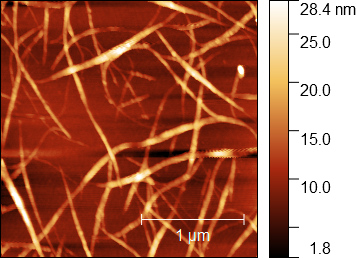
\includegraphics{figures/ch5/Ned_NTQ24_20220125_00235.png}

}

}

\end{minipage}%
%
\begin{minipage}[t]{0.01\linewidth}

{\centering 

~

}

\end{minipage}%
%
\begin{minipage}[t]{0.03\linewidth}

{\centering 

\raisebox{-\height}{

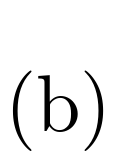
\includegraphics{figures/(b).png}

}

}

\end{minipage}%
%
\begin{minipage}[t]{0.01\linewidth}

{\centering 

~

}

\end{minipage}%
%
\begin{minipage}[t]{0.45\linewidth}

{\centering 

\raisebox{-\height}{

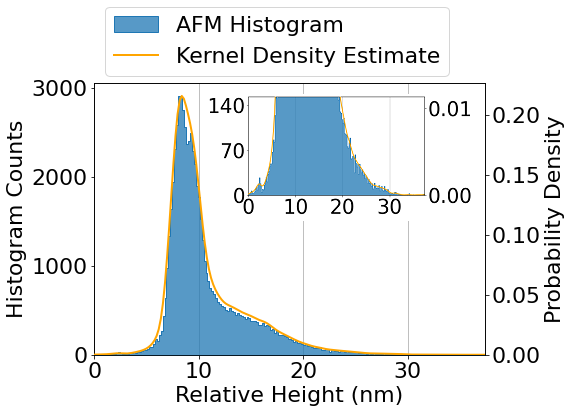
\includegraphics{figures/ch5/Ned_NTQ24_20220125_00235_histogram_initialguess_inset.png}

}

}

\end{minipage}%
%
\begin{minipage}[t]{0.01\linewidth}

{\centering 

~

}

\end{minipage}%
\newline
\begin{minipage}[t]{0.03\linewidth}

{\centering 

\raisebox{-\height}{


\includegraphics{figures/(c).png}

}

}

\end{minipage}%
%
\begin{minipage}[t]{0.01\linewidth}

{\centering 

~

}

\end{minipage}%
%
\begin{minipage}[t]{0.45\linewidth}

{\centering 

\raisebox{-\height}{

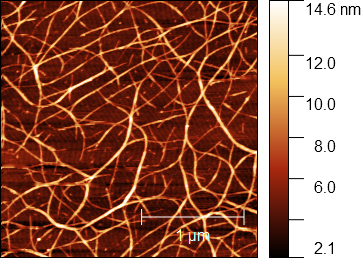
\includegraphics{figures/ch5/Ned_NTQ8C7_w4_pristine_00084_20210428(2).png}

}

}

\end{minipage}%
%
\begin{minipage}[t]{0.01\linewidth}

{\centering 

~

}

\end{minipage}%
%
\begin{minipage}[t]{0.03\linewidth}

{\centering 

\raisebox{-\height}{

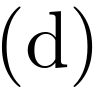
\includegraphics{figures/(d).png}

}

}

\end{minipage}%
%
\begin{minipage}[t]{0.01\linewidth}

{\centering 

~

}

\end{minipage}%
%
\begin{minipage}[t]{0.45\linewidth}

{\centering 

\raisebox{-\height}{

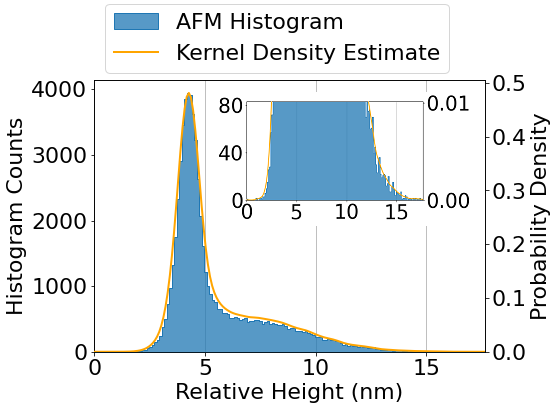
\includegraphics{figures/ch5/Ned_NTQ8C7_w4_pristine_00084_20210428(2)_histogram_initialguess_inset.png}

}

}

\end{minipage}%
%
\begin{minipage}[t]{0.01\linewidth}

{\centering 

~

}

\end{minipage}%
\newline
\begin{minipage}[t]{0.03\linewidth}

{\centering 

\raisebox{-\height}{

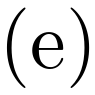
\includegraphics{figures/(e).png}

}

}

\end{minipage}%
%
\begin{minipage}[t]{0.01\linewidth}

{\centering 

~

}

\end{minipage}%
%
\begin{minipage}[t]{0.45\linewidth}

{\centering 

\raisebox{-\height}{

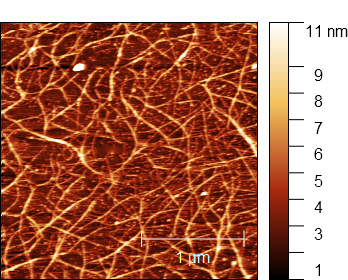
\includegraphics{figures/ch5/Ned_NGQ14D2_W4_pristine_20220713_00567.png}

}

}

\end{minipage}%
%
\begin{minipage}[t]{0.01\linewidth}

{\centering 

~

}

\end{minipage}%
%
\begin{minipage}[t]{0.03\linewidth}

{\centering 

\raisebox{-\height}{

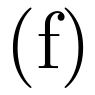
\includegraphics{figures/(f).png}

}

}

\end{minipage}%
%
\begin{minipage}[t]{0.01\linewidth}

{\centering 

~

}

\end{minipage}%
%
\begin{minipage}[t]{0.45\linewidth}

{\centering 

\raisebox{-\height}{

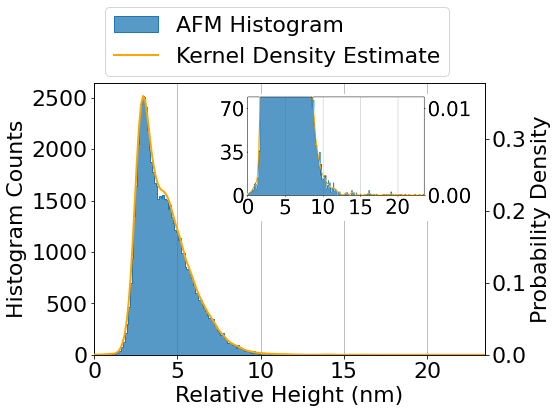
\includegraphics{figures/ch5/Ned_NGQ14D2_W4_pristine_20220713_00567_histogram_initialguess_inset.png}

}

}

\end{minipage}%
%
\begin{minipage}[t]{0.01\linewidth}

{\centering 

~

}

\end{minipage}%

\caption{\label{fig-afm-morphology}2.5 µm \(\times\) 2.5 µm atomic force
microscope (AFM) images of carbon nanotube films deposited using various
methods, shown side-by-side with histogram height distributions and
kernel density estimate (KDE) plots corresponding to each image. The
network shown in (a) with height distribution shown in (b) was deposited
in solvent, the network shown in (c) with height distribution shown in
(d) was dropcast in surfactant, and the network shown in (e) with height
distribution shown in (f) was dropcast in surfactant with steam
present.}

\end{figure}

It has previously been demonstrated that the diameter range of deposited
single-walled carbon nanotubes can be modelled via a normal or Gaussian
distribution \autocite{LeMieux2008,Liu2013,Vobornik2023}. However, when
the height profiles from the 2.5 µm \(\times\) 2.5 µm AFM images are
directly extracted and binned, as shown in
Figure~\ref{fig-afm-morphology}, the histograms obtained do not follow a
normal distribution. One reason for this result is that the carbon
nanotubes do not lie perfectly flat on the substrate surface, as the
SiO\(_2\) substrate and the carbon nanotubes each possess some surface
roughness. To find the contribution of substrate surface roughness to
the height profile histogram corresponding to each network deposition
method, SiO\(_2\) substrates were modified using the same processes as
in Figure~\ref{fig-afm-morphology} but without carbon nanotubes present
in the solutions used. 2.5 µm \(\times\) 2.5 µm AFM images of the
modified surfaces are shown in Figure~\ref{fig-afm-substrate}.

\begin{figure}

\begin{minipage}[t]{0.03\linewidth}

{\centering 

\raisebox{-\height}{


\includegraphics{figures/(a).png}

}

}

\end{minipage}%
%
\begin{minipage}[t]{0.01\linewidth}

{\centering 

~

}

\end{minipage}%
%
\begin{minipage}[t]{0.45\linewidth}

{\centering 

\raisebox{-\height}{

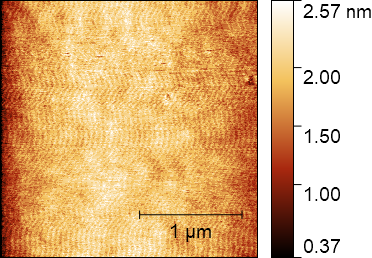
\includegraphics{figures/ch5/Ned_SiO2_00351_20231016.png}

}

}

\end{minipage}%
%
\begin{minipage}[t]{0.01\linewidth}

{\centering 

~

}

\end{minipage}%
%
\begin{minipage}[t]{0.03\linewidth}

{\centering 

\raisebox{-\height}{

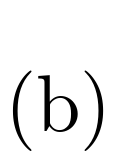
\includegraphics{figures/(b).png}

}

}

\end{minipage}%
%
\begin{minipage}[t]{0.01\linewidth}

{\centering 

~

}

\end{minipage}%
%
\begin{minipage}[t]{0.45\linewidth}

{\centering 

\raisebox{-\height}{

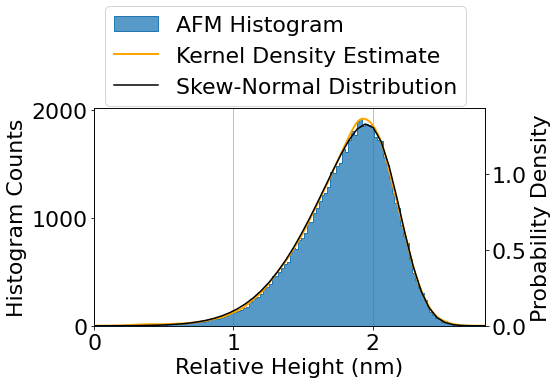
\includegraphics{figures/ch5/Ned_SiO2_00351_20231016_histogram_initialguess.png}

}

}

\end{minipage}%
%
\begin{minipage}[t]{0.01\linewidth}

{\centering 

~

}

\end{minipage}%
\newline
\begin{minipage}[t]{0.03\linewidth}

{\centering 

\raisebox{-\height}{


\includegraphics{figures/(c).png}

}

}

\end{minipage}%
%
\begin{minipage}[t]{0.01\linewidth}

{\centering 

~

}

\end{minipage}%
%
\begin{minipage}[t]{0.45\linewidth}

{\centering 

\raisebox{-\height}{

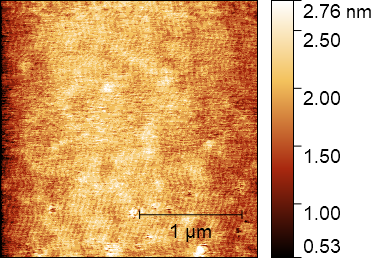
\includegraphics{figures/ch5/Ned_SiO2_s_surfactant_nosteam_00355_20231016.png}

}

}

\end{minipage}%
%
\begin{minipage}[t]{0.01\linewidth}

{\centering 

~

}

\end{minipage}%
%
\begin{minipage}[t]{0.03\linewidth}

{\centering 

\raisebox{-\height}{

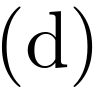
\includegraphics{figures/(d).png}

}

}

\end{minipage}%
%
\begin{minipage}[t]{0.01\linewidth}

{\centering 

~

}

\end{minipage}%
%
\begin{minipage}[t]{0.45\linewidth}

{\centering 

\raisebox{-\height}{

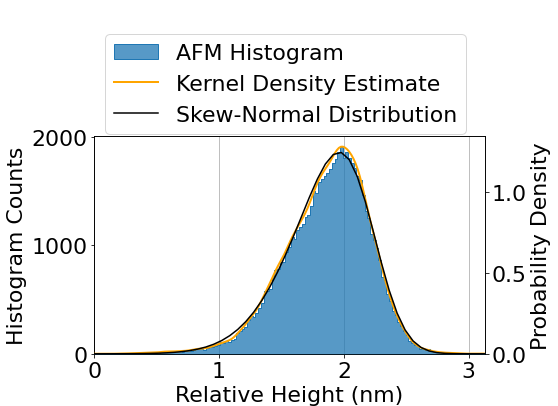
\includegraphics{figures/ch5/Ned_SiO2_s_surfactant_nosteam_00355_20231016_histogram_initialguess.png}

}

}

\end{minipage}%
%
\begin{minipage}[t]{0.01\linewidth}

{\centering 

~

}

\end{minipage}%
\newline
\begin{minipage}[t]{0.03\linewidth}

{\centering 

\raisebox{-\height}{

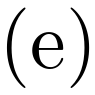
\includegraphics{figures/(e).png}

}

}

\end{minipage}%
%
\begin{minipage}[t]{0.01\linewidth}

{\centering 

~

}

\end{minipage}%
%
\begin{minipage}[t]{0.45\linewidth}

{\centering 

\raisebox{-\height}{

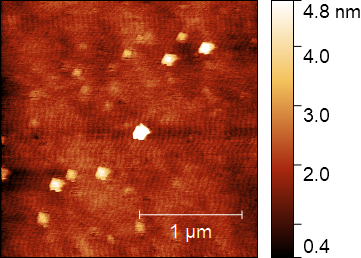
\includegraphics{figures/ch5/Ned_SiO2_s_surfactant_steam_00357_20231016.png}

}

}

\end{minipage}%
%
\begin{minipage}[t]{0.01\linewidth}

{\centering 

~

}

\end{minipage}%
%
\begin{minipage}[t]{0.03\linewidth}

{\centering 

\raisebox{-\height}{

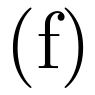
\includegraphics{figures/(f).png}

}

}

\end{minipage}%
%
\begin{minipage}[t]{0.01\linewidth}

{\centering 

~

}

\end{minipage}%
%
\begin{minipage}[t]{0.45\linewidth}

{\centering 

\raisebox{-\height}{

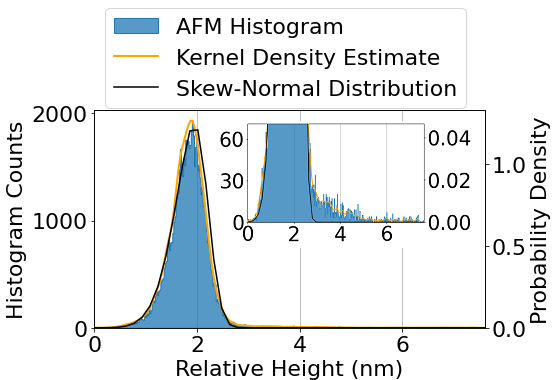
\includegraphics{figures/ch5/Ned_SiO2_s_surfactant_steam_00357_20231016_histogram_initialguess_inset.png}

}

}

\end{minipage}%
%
\begin{minipage}[t]{0.01\linewidth}

{\centering 

~

}

\end{minipage}%

\caption{\label{fig-afm-substrate}2.5 µm \(\times\) 2.5 µm atomic force
microscope (AFM) images of SiO\(_2\) substrates alongside histogram
height distributions and KDE plots corresponding to each image. The
substrate in (a) and (b) was exposed to solvent, the substrate in (c)
and (d) was exposed to surfactant, and the substrate in (e) and (f) was
exposed to surfactant with steam present. The inset in (f) shows the
long tail due to surfactant.}

\end{figure}

\begin{equation}\protect\hypertarget{eq-skew}{}{
f(x) = 2\phi(x)\Phi(\alpha x)
}\label{eq-skew}\end{equation}

In Figure~\ref{fig-afm-substrate}, it appears that each substrate
surface has a roughness that follows a normal distribution with some
degree of skewness. Figure~\ref{fig-afm-substrate} (b) and
Figure~\ref{fig-afm-substrate} (d) are negatively skewed distributions.
The equation for a skew-normal distribution is given in
Equation~\ref{eq-skew}, where \(\alpha\) is the `slant parameter' which
indicates the skewness of the distribution, \(\phi(x)\) is the standard
normal distribution and \(\Phi(x)\) is the corresponding cumulative
distribution function. To modify this distribution for the most general
case, the `location parameter' \(\xi\) and `scale parameter' \(\omega\)
are introduced, which correspond to the mean and standard deviation of
the skew-free normal distribution when \(\alpha\) is set equal to zero.
These parameters are inserted into Equation~\ref{eq-skew} by setting
\(x \rightarrow (x-\xi)/\omega\) and replacing the factor 2 with
\(2/\omega\) \autocite{Azzalini2013}. The fitted skew-normal
distribution in Figure~\ref{fig-afm-substrate} (b) has
\(\alpha = -3.2\), \(\xi = 2.2\) nm and \(\omega = 0.5\) nm, while in
Figure~\ref{fig-afm-substrate} (d) \(\alpha = -2.2\), \(\xi = 2.2\) nm
and \(\omega = 0.5\) nm. The close correspondence between \(\xi\) and
\(\omega\) for these distributions implies that the skewness is a
variable imaging or processing artifact rather than a physical property
of the surface. Without distortion, the roughness of a clean SiO\(_2\)
surface should follow a normal distribution \autocite{Velicky2015}.

Figure~\ref{fig-afm-substrate} (f) has a pronounced positive skew
\(\sim\) 5.5 nm in length. The tail results from the droplets observed
in Figure~\ref{fig-afm-substrate} (e), which may be condensation from
the steam or surfactant residue trapped by the steam environment
\autocite{Christensen2022,Vobornik2023}. Attempting to fit a skew-normal
distribution to this histogram fails when all three variables are
allowed to vary due to the presence of the tail. Instead, previous
values obtained for \(\xi\) and \(\omega\) can be set fixed at \(\xi\)
and \(\omega\) at 2.2 nm and 0.5 nm respectively in the fitting process,
assuming that these values are characteristic of the imaging process
used and not the substrate. In this fitting process, therefore, only
\(\alpha\) was allowed to change. The resulting fitted distribution is
shown in Figure~\ref{fig-afm-substrate} (f), with \(\alpha = -2.4\). The
distribution closely fits the negative tail of the histogram, but
deviates from the positive tail due to the presence of the droplets.
This deviation is small and the fit is otherwise good quality, with an
R-squared value of 0.98. If the contamination identified here is
surfactant, this could have negative effects on both sensitivity of
carbon nanotubes and also could damage the attached biological elements.

\begin{figure}

\begin{minipage}[t]{0.03\linewidth}

{\centering 

\raisebox{-\height}{


\includegraphics{figures/(a).png}

}

}

\end{minipage}%
%
\begin{minipage}[t]{0.01\linewidth}

{\centering 

~

}

\end{minipage}%
%
\begin{minipage}[t]{0.45\linewidth}

{\centering 

\raisebox{-\height}{

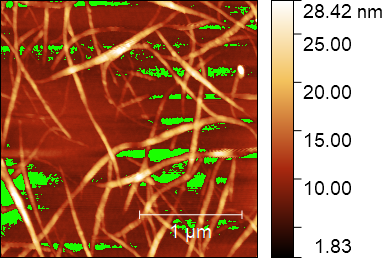
\includegraphics{figures/ch5/Ned_NTQ24_20220125_00235_artifacts.png}

}

}

\end{minipage}%
%
\begin{minipage}[t]{0.01\linewidth}

{\centering 

~

}

\end{minipage}%
%
\begin{minipage}[t]{0.03\linewidth}

{\centering 

\raisebox{-\height}{

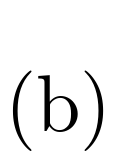
\includegraphics{figures/(b).png}

}

}

\end{minipage}%
%
\begin{minipage}[t]{0.01\linewidth}

{\centering 

~

}

\end{minipage}%
%
\begin{minipage}[t]{0.45\linewidth}

{\centering 

\raisebox{-\height}{

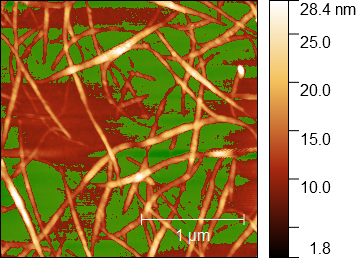
\includegraphics{figures/ch5/Ned_NTQ24_20220125_00235_2.png}

}

}

\end{minipage}%
%
\begin{minipage}[t]{0.01\linewidth}

{\centering 

~

}

\end{minipage}%
\newline
\begin{minipage}[t]{0.03\linewidth}

{\centering 

\raisebox{-\height}{


\includegraphics{figures/(c).png}

}

}

\end{minipage}%
%
\begin{minipage}[t]{0.01\linewidth}

{\centering 

~

}

\end{minipage}%
%
\begin{minipage}[t]{0.45\linewidth}

{\centering 

\raisebox{-\height}{

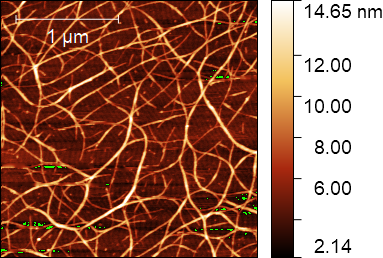
\includegraphics{figures/ch5/Ned_NTQ8C7_w4_pristine_00084_20210428(2)_artifacts.png}

}

}

\end{minipage}%
%
\begin{minipage}[t]{0.01\linewidth}

{\centering 

~

}

\end{minipage}%
%
\begin{minipage}[t]{0.03\linewidth}

{\centering 

\raisebox{-\height}{

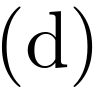
\includegraphics{figures/(d).png}

}

}

\end{minipage}%
%
\begin{minipage}[t]{0.01\linewidth}

{\centering 

~

}

\end{minipage}%
%
\begin{minipage}[t]{0.45\linewidth}

{\centering 

\raisebox{-\height}{

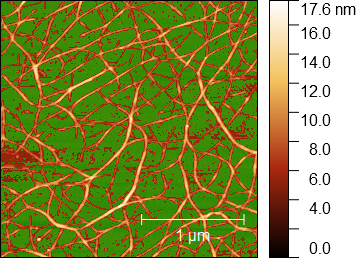
\includegraphics{figures/ch5/Ned_NTQ8C7_w4_pristine_00084_20210428(2)_2.png}

}

}

\end{minipage}%
%
\begin{minipage}[t]{0.01\linewidth}

{\centering 

~

}

\end{minipage}%
\newline
\begin{minipage}[t]{0.03\linewidth}

{\centering 

\raisebox{-\height}{

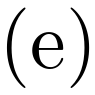
\includegraphics{figures/(e).png}

}

}

\end{minipage}%
%
\begin{minipage}[t]{0.01\linewidth}

{\centering 

~

}

\end{minipage}%
%
\begin{minipage}[t]{0.45\linewidth}

{\centering 

\raisebox{-\height}{

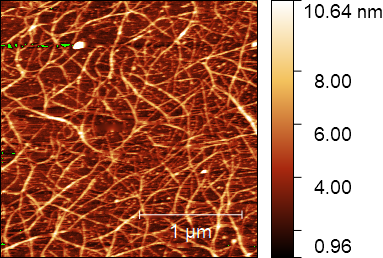
\includegraphics{figures/ch5/Ned_NGQ14D2_W4_pristine_20220713_00567_artifacts.png}

}

}

\end{minipage}%
%
\begin{minipage}[t]{0.01\linewidth}

{\centering 

~

}

\end{minipage}%
%
\begin{minipage}[t]{0.03\linewidth}

{\centering 

\raisebox{-\height}{

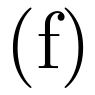
\includegraphics{figures/(f).png}

}

}

\end{minipage}%
%
\begin{minipage}[t]{0.01\linewidth}

{\centering 

~

}

\end{minipage}%
%
\begin{minipage}[t]{0.45\linewidth}

{\centering 

\raisebox{-\height}{

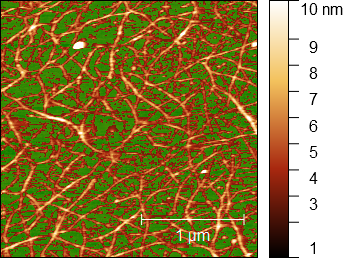
\includegraphics{figures/ch5/Ned_NGQ14D2_W4_pristine_20220713_00567_2.png}

}

}

\end{minipage}%
%
\begin{minipage}[t]{0.01\linewidth}

{\centering 

~

}

\end{minipage}%

\caption{\label{fig-cnt-mask}A mask, shaded green, sets a height
threshold so that masked features are hidden from the height dataset.
The network in (a)-(b) was solvent-deposited, the network in (c)-(d)
surfactant-deposited, and the network in (e)-(f) surfactant-deposited
with steam present. Height thresholds have been chosen so that deep
trough-like artifacts are masked in (a), (c) and (e), while height
thresholds which exclude the full average background height of each
network are shown in (b), (d) and (f).}

\end{figure}

Following the morphology analysis technique outlined by Vobornik
\emph{et al.} \autocite{Vobornik2023}, background values were found
which corresponded to the substrate roughness of each network. Taking
the average of each substrate surface height corresponding to
solvent-deposition, surfactant-deposition and steam-assisted
surfactant-deposition films gave values of \(1.8 \pm 0.3\) nm,
\(1.9 \pm 0.3\) nm and \(1.8 \pm 0.5\) nm respectively. From
Figure~\ref{fig-afm-morphology}, it is also apparent that measuring
relatively large features with the atomic force microscope leads to deep
image artifacts in the vicinity of these features which appear as
rounded streaks unrelated to surface roughness. These artifacts have
been highlighted for the solvent-deposition, surfactant-deposition and
steam-assisted surfactant-deposition films using a coloured height
threshold or `mask' added with the Gwyddion software package in
Figure~\ref{fig-cnt-mask} (a), Figure~\ref{fig-cnt-mask} (c) and
Figure~\ref{fig-cnt-mask} (e). The maximum artifact height in each
figure was \(6.3 \pm 0.7\) nm, \(2.6 \pm 0.3\) nm and \(0.9 \pm 0.3\)
nm. By adding the median substrate height to the maximum artifact
height, the mean background value can be found. This value can be used
to distinguish the carbon nanotube bundles in the network from the
substrate, demonstrated for each background value with a Gwyddion mask
in Figure~\ref{fig-cnt-mask} (b), Figure~\ref{fig-cnt-mask} (d) and
Figure~\ref{fig-cnt-mask} (f).

\begin{figure}

\begin{minipage}[t]{0.03\linewidth}

{\centering 

\raisebox{-\height}{


\includegraphics{figures/(a).png}

}

}

\end{minipage}%
%
\begin{minipage}[t]{0.01\linewidth}

{\centering 

~

}

\end{minipage}%
%
\begin{minipage}[t]{0.45\linewidth}

{\centering 

\raisebox{-\height}{

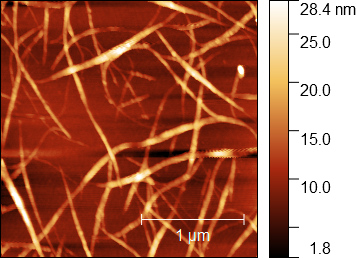
\includegraphics{figures/ch5/Ned_NTQ24_20220125_00235.png}

}

}

\end{minipage}%
%
\begin{minipage}[t]{0.01\linewidth}

{\centering 

~

}

\end{minipage}%
%
\begin{minipage}[t]{0.03\linewidth}

{\centering 

\raisebox{-\height}{

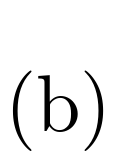
\includegraphics{figures/(b).png}

}

}

\end{minipage}%
%
\begin{minipage}[t]{0.01\linewidth}

{\centering 

~

}

\end{minipage}%
%
\begin{minipage}[t]{0.45\linewidth}

{\centering 

\raisebox{-\height}{

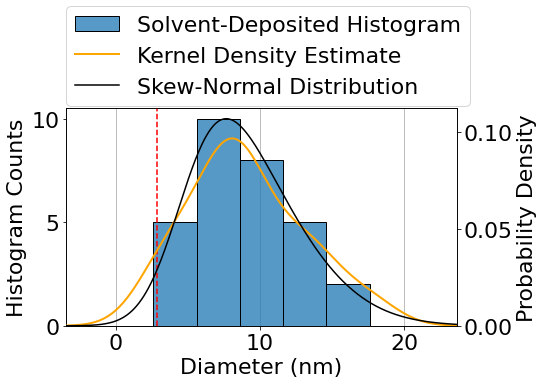
\includegraphics{figures/ch5/NTQ24_20220125_00235_cnt_histogram.png}

}

}

\end{minipage}%
%
\begin{minipage}[t]{0.01\linewidth}

{\centering 

~

}

\end{minipage}%
\newline
\begin{minipage}[t]{0.03\linewidth}

{\centering 

\raisebox{-\height}{


\includegraphics{figures/(c).png}

}

}

\end{minipage}%
%
\begin{minipage}[t]{0.01\linewidth}

{\centering 

~

}

\end{minipage}%
%
\begin{minipage}[t]{0.45\linewidth}

{\centering 

\raisebox{-\height}{

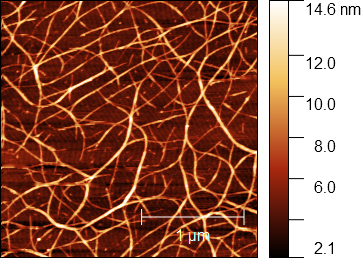
\includegraphics{figures/ch5/Ned_NTQ8C7_w4_pristine_00084_20210428(2).png}

}

}

\end{minipage}%
%
\begin{minipage}[t]{0.01\linewidth}

{\centering 

~

}

\end{minipage}%
%
\begin{minipage}[t]{0.03\linewidth}

{\centering 

\raisebox{-\height}{

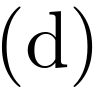
\includegraphics{figures/(d).png}

}

}

\end{minipage}%
%
\begin{minipage}[t]{0.01\linewidth}

{\centering 

~

}

\end{minipage}%
%
\begin{minipage}[t]{0.45\linewidth}

{\centering 

\raisebox{-\height}{

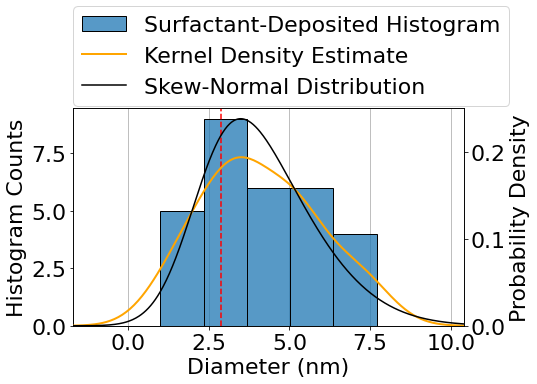
\includegraphics{figures/ch5/NTQ8C7_w4_pristine_cnt_histogram.png}

}

}

\end{minipage}%
%
\begin{minipage}[t]{0.01\linewidth}

{\centering 

~

}

\end{minipage}%
\newline
\begin{minipage}[t]{0.03\linewidth}

{\centering 

\raisebox{-\height}{

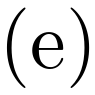
\includegraphics{figures/(e).png}

}

}

\end{minipage}%
%
\begin{minipage}[t]{0.01\linewidth}

{\centering 

~

}

\end{minipage}%
%
\begin{minipage}[t]{0.45\linewidth}

{\centering 

\raisebox{-\height}{

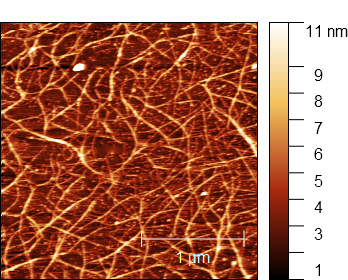
\includegraphics{figures/ch5/Ned_NGQ14D2_W4_pristine_20220713_00567.png}

}

}

\end{minipage}%
%
\begin{minipage}[t]{0.01\linewidth}

{\centering 

~

}

\end{minipage}%
%
\begin{minipage}[t]{0.03\linewidth}

{\centering 

\raisebox{-\height}{

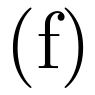
\includegraphics{figures/(f).png}

}

}

\end{minipage}%
%
\begin{minipage}[t]{0.01\linewidth}

{\centering 

~

}

\end{minipage}%
%
\begin{minipage}[t]{0.45\linewidth}

{\centering 

\raisebox{-\height}{

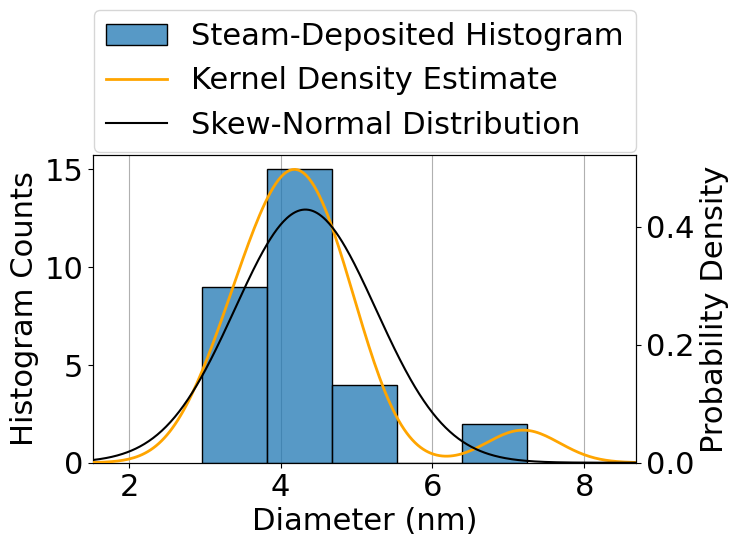
\includegraphics{figures/ch5/NT14D2_W4_pristine_cnt_histogram.png}

}

}

\end{minipage}%
%
\begin{minipage}[t]{0.01\linewidth}

{\centering 

~

}

\end{minipage}%

\caption{\label{fig-cnt-histogram}Histogram height distributions for
each carbon nanotube network with corresponding kernel density estimate
plots collected via the morphology analysis method outlined by Vobornik
\emph{et al.} \autocite{Vobornik2023}. The histogram for the
solvent-deposited network in (a) is shown in (b), the histogram for the
surfactant-deposited network in (c) is shown in (d), and the histogram
for the steam-assisted surfactant-deposited network shown in (e) is
shown in (f). The red dotted line represents the lower bound for
multi-tube bundles, assuming the minimum nanotube diameter is 1.45 nm.}

\end{figure}

Five successive diameter measurements of 30 carbon nanotube bundles were
collected using Gwyddion. Measurements were not taken at bundle
junctions. The average of five values for each carbon nanotube bundle
was then taken and the corresponding background height of the substrate
subtracted. The 30 height values were sorted into five equal-sized bins,
as shown in Figure~\ref{fig-cnt-histogram}. Each histogram appears to
follow a moderately positive-skewed normal distribution, different to
the skew-free normal distribution found in previous works
\autocite{LeMieux2008,Liu2013,Vobornik2023}. The skew is likely to be
another imaging artifact. The force of the atomic force microscope tip
is known to cause larger bundles to undergo some degree of compression,
and the resulting systematic underestimation of their height may be
responsible for the distribution skewness \autocite{Vobornik2023}. The
fitted skew-normal distribution in Figure~\ref{fig-cnt-histogram} (b)
has \(\alpha = 2.5\) (slant, indicates skew), \(\xi = 4.7\) nm
(location, indicates mean), \(\omega = 5.9\) nm (scale, indicates
standard deviation), the distribution in Figure~\ref{fig-cnt-histogram}
(c) has \(\alpha = 2.4\), \(\xi = 2.2\) nm, \(\omega = 2.6\) nm, and the
distribution in Figure~\ref{fig-cnt-histogram} (d) has \(\alpha = 3.5\),
\(\xi = 2.9\) nm and \(\omega = 1.5\) nm. The probability density for
the carbon nanotube bundle histogram drops to approximately zero at or
before 0 nm, indicating each fit is physically realistic.

Analysis of carbon nanotube network morphology can be simplified by
assuming the component nanotubes are cylinders, follow 2D packing and
are of equal diameter \autocite{Murugathas2018}.
Table~\ref{tbl-circle-packing} shows the relationship between the
diameter of a bundle of 2D packed cylinders and their constituent
diameters. By using the relevant \(d\)/\(d_n\) packing ratio, and
assuming an average carbon nanotube diameter of 1.45 nm, it is possible
to use Table~\ref{tbl-circle-packing} to find the approximate number of
nanotubes \emph{n} likely to be present in the simple average bundle
size corresponding to each deposition type
\autocite{Graham1998,Specht2023}. These estimates are shown in
Table~\ref{tbl-histogram-parameters}. Also shown in
Table~\ref{tbl-histogram-parameters} is an estimate of the ratio of
single- to multi-tube bundles for each deposition. This estimate was
obtained by taking the integral of each probability distribution with a
lower bound of 2.9 nm, the minimum multi-tube bundle size for 1.45 nm
diameter nanotubes, indicated with a red dotted line in
Figure~\ref{fig-cnt-histogram}. As the area under the curve represents
the probability a bundle will have a particular diameter, the ratio of
this integral to the integral over the entire interval should give a
reasonable estimate of the relative proportion of multi-tube bundles.
Table~\ref{tbl-histogram-parameters} should be interpreted as
lower-limit estimates, remembering that bundle sizes are likely being
underestimated \autocite{Vobornik2023}.

\hypertarget{tbl-circle-packing}{}
\begin{longtable}[]{@{}
  >{\raggedright\arraybackslash}p{(\columnwidth - 16\tabcolsep) * \real{0.1053}}
  >{\raggedright\arraybackslash}p{(\columnwidth - 16\tabcolsep) * \real{0.1228}}
  >{\raggedright\arraybackslash}p{(\columnwidth - 16\tabcolsep) * \real{0.0965}}
  >{\raggedright\arraybackslash}p{(\columnwidth - 16\tabcolsep) * \real{0.0965}}
  >{\raggedright\arraybackslash}p{(\columnwidth - 16\tabcolsep) * \real{0.1228}}
  >{\raggedright\arraybackslash}p{(\columnwidth - 16\tabcolsep) * \real{0.1228}}
  >{\raggedright\arraybackslash}p{(\columnwidth - 16\tabcolsep) * \real{0.1228}}
  >{\raggedright\arraybackslash}p{(\columnwidth - 16\tabcolsep) * \real{0.1228}}
  >{\raggedright\arraybackslash}p{(\columnwidth - 16\tabcolsep) * \real{0.0877}}@{}}
\caption{\label{tbl-circle-packing}The first eight optimised ratios of
2D packed circle diameter to encompassing circle diameter, given to 3
s.f. (encompassing circle diameter = \(d\), number of packed circles =
\(n\), approximate packed circle diameter = \(d_n\)).\\
}\tabularnewline
\toprule\noalign{}
\endfirsthead
\endhead
\bottomrule\noalign{}
\endlastfoot
\(n\) & \text{2} & \text{3} & \text{4} & \text{5} & \text{6} & \text{7}
& \text{8} & \text{9} \\
\(d\)/\(d_n\) & \text{2.00} & 2.15 & 2.41 & \text{2.70} & \text{3.00} &
\text{3.00} & \text{3.30} & 3.61 \\
\end{longtable}

Both the carbon nanotube bundle diameter mean and standard deviation are
small for surfactant-deposited films when compared to the mean and
standard deviation of solvent-deposited films. However, despite the
presence of surfactant, it is apparent both from
Figure~\ref{fig-cnt-histogram} and Table~\ref{tbl-histogram-parameters}
that most surfactant-dispersed carbon nanotubes are not deposited
individually. It is possible that the bundling of surfactant-dispersed
carbon nanotubes occurs as nanotubes are deposited onto the surface, as
this bonding process may disrupt the repulsive forces from the
surfactant coating and allow attractive forces to temporarily dominate.
Interestingly, the presence of steam appears to slightly increase the
size of bundles. It may be the case that steam further disrupts the
repulsive forces from the surfactant. Alternatively, the larger bundle
sizes measured may partly consist of water vapour adsorbed to the
surface of the carbon nanotubes during the deposition process.

The surface coverage values for each network are shown in
Table~\ref{tbl-histogram-parameters}, found by comparing the surface
area of the masked area in Figure~\ref{fig-cnt-mask} with the full image
surface area. These values show that introducing steam to the surfactant
deposition process doubles the surface coverage of the SiO\(_2\)
substrate by the carbon nanotubes. The relatively low surface coverage
seen in Figure~\ref{fig-cnt-histogram} (c) can be explained by the
coffee-ring effect. The coffee-ring effect refers to a build-up of
dispersed solid forming around the edges of a dispersion evaporating on
a surface. The dispersion edges are fixed by surface forces, leading to
capillary flow outwards to replace liquid evaporating at the edges,
which carries solid material alongside
\autocite{Deegan1997,VanGaalen2021}. Water vapour is known to disrupt
this capillary effect \autocite{Bishop2020}, which reduces the flow of
carbon nanotubes to the edges of the substrate. A reduction in the
coffee-ring effect leads to carbon nanotubes being deposited more evenly
across the surface of the substrate. A even surface coverage gives a
denser network on average, explaining the denser network seen in
Figure~\ref{fig-cnt-histogram} (e).

\hypertarget{tbl-histogram-parameters}{}
\begin{longtable}[t]{>{\raggedright\arraybackslash}p{3.5cm}>{\centering\arraybackslash}p{2.2cm}>{\centering\arraybackslash}p{2.2cm}>{\centering\arraybackslash}p{2.2cm}>{\centering\arraybackslash}p{2.2cm}}
\caption{\label{tbl-histogram-parameters}The mean of histogram distributions for carbon nanotube films deposited
using various methods, alongside estimates for the number of nanotubes
present per mean bundle, the estimated proportion of multi-tube bundles
present across the network and the proportion of substrate covered by
the nanotubes. }\tabularnewline

\toprule
 & Mean Bundle Diameter (nm) & Tubes per Average Bundle & \% Multi-Tube Bundles & \% Nanotube Coverage\\
\midrule
Solvent deposited & 9.1 ± 4.0 & 30 & > 97\% & < 50\%\\
Surfactant deposited & 4.1 ± 1.8 & 5 & > 74\% & 35\%\\
Surfactant deposited with steam & 4.0 ± 1.0 & 5 & > 91\% & 70\%\\
\bottomrule
\end{longtable}

The discussion in this section gives us a new understanding of the
histograms shown in Figure~\ref{fig-afm-morphology}. It appears that
these histograms are linear combinations of skewed normal distributions.
These distributions include a negatively-skewed distribution
corresponding to the substrate surface and a positively-skewed
distribution corresponding to the carbon nanotube bundles. The
trough-like image artifacts as well as X and Y junctions between
overlapping nanotubes may also form similarly skewed normal
distributions as part of the complete image histogram
\autocite{Murugathas2018}. The linear combination of histograms could be
modelled mathematically in order to rapidly extract key parameters from
atomic force microscope images \autocite{Marchenko2010}, but
implementing this approach is outside of the scope of this thesis.
Introducing steam when depositing with surfactant increases the density
of network deposition, but also leads to increased adsorption of water
and possibly surfactant onto the substrate and network. Finding a method
of removing the unwanted surfactant present may be required for robust
biosensors \autocite{Kane2014,Barnett2018}.

\hypertarget{sec-pristine-raman}{%
\subsection{Raman Spectroscopy}\label{sec-pristine-raman}}

Raman spectroscopy was also used to analyse and compare the deposited
carbon nanotube networks. Raman spectra were collected from a
solvent-deposited carbon nanotube film and a steam-assisted
surfactant-deposited film, both on SiO\(_2\), in the manner described in
\textbf{?@sec-raman-characterisation}. These spectra were then processed
using the Python script mentioned in Section~\ref{sec-raman-analysis}.
For each location, spectra over two wavenumber ranges were collected. A
peak corresponding to the SiO\(_2\) substrate, found in the range
between 100 cm\(^{-1}\) and 650 cm\(^{-1}\), was used as a reference
peak for the normalisation of intensity across the wavenumber range
between 1300 cm\(^{-1}\) and 1650 cm\(^{-1}\). These normalised spectra
are shown in Figure~\ref{fig-pristine-raman}. In all spectra, a D-band
comprising a single D-peak is observed at \(\sim\) 1320 cm\(^{-1}\), and
a G-band comprising two G-peaks, G\(^-\) and G\(^+\), is observed
between \(\sim\) 1525 cm\(^{-1}\) and \(\sim\) 1650 cm\(^{-1}\). These
features are characteristic of networks of semiconducting carbon
nanotubes \autocite{Dresselhaus2005,King2014}.

\begin{figure}

\begin{minipage}[t]{0.11\linewidth}

{\centering 

~

}

\end{minipage}%
%
\begin{minipage}[t]{0.03\linewidth}

{\centering 

\raisebox{-\height}{


\includegraphics{figures/(a).png}

}

}

\end{minipage}%
%
\begin{minipage}[t]{0.01\linewidth}

{\centering 

~

}

\end{minipage}%
%
\begin{minipage}[t]{0.70\linewidth}

{\centering 

\raisebox{-\height}{

\includegraphics{figures/ch5/bundled_raman.png}

}

}

\end{minipage}%
%
\begin{minipage}[t]{0.15\linewidth}

{\centering 

~

}

\end{minipage}%
\newline
\begin{minipage}[t]{0.11\linewidth}

{\centering 

~

}

\end{minipage}%
%
\begin{minipage}[t]{0.03\linewidth}

{\centering 

\raisebox{-\height}{

\includegraphics{figures/(b).png}

}

}

\end{minipage}%
%
\begin{minipage}[t]{0.01\linewidth}

{\centering 

~

}

\end{minipage}%
%
\begin{minipage}[t]{0.70\linewidth}

{\centering 

\raisebox{-\height}{

\includegraphics{figures/ch5/singletube_raman.png}

}

}

\end{minipage}%
%
\begin{minipage}[t]{0.15\linewidth}

{\centering 

~

}

\end{minipage}%
\newline
\begin{minipage}[t]{0.10\linewidth}

{\centering 

~

}

\end{minipage}%
%
\begin{minipage}[t]{0.03\linewidth}

{\centering 

\raisebox{-\height}{

\includegraphics{figures/(c).png}

}

}

\end{minipage}%
%
\begin{minipage}[t]{0.01\linewidth}

{\centering 

~

}

\end{minipage}%
%
\begin{minipage}[t]{0.72\linewidth}

{\centering 

\raisebox{-\height}{

\includegraphics{figures/ch5/comparison-raman.png}

}

}

\end{minipage}%
%
\begin{minipage}[t]{0.14\linewidth}

{\centering 

~

}

\end{minipage}%

\caption{\label{fig-pristine-raman}A series of nine Raman spectra at
different locations across a 40 µm \(\times\) 100 µm carbon nanotube
film region, where (a) shows spectra from a film deposited using solvent
while (b) shows spectra from a film deposited with surfactant in the
presence of steam. (c) shows a histogram of the range of
D-peak/G\(^+\)-peak spectral ratios corresponding to each film.}

\end{figure}

Closer inspection of the D-peak and G-peaks in
Figure~\ref{fig-pristine-raman} can give us important information about
network composition. G\(^-\) is a minor peak found at \(\sim\) 1570
cm\(^{-1}\), while G\(^+\) is a larger feature at \(\sim\) 1590
cm\(^{-1}\). The G\(^+\) feature describes the in-plane vibration of
carbon bonds along the length of the carbon nanotubes, while the G\(^-\)
feature describes the in-plane vibration of bonds about the nanotube
circumference \autocite{King2014,Swiniarski2021}. The splitting between
the wavenumber location of the G\(^-\) and G\(^+\) local maxima is lower
in Figure~\ref{fig-pristine-raman} (b) than in
Figure~\ref{fig-pristine-raman} (a), indicating more metallic nanotubes
are present in the surfactant-deposited network
\autocite{Swiniarski2021}. The D-peak gives an indication of the defects
present in the carbon nanotube atomic structure
\autocite{King2014,Swiniarski2021}. The size of the normalised D-peak
appears much lower in Figure~\ref{fig-pristine-raman} (a) than in
Figure~\ref{fig-pristine-raman} (b), indicating the solvent deposition
process introduces less defects to the carbon nanotubes than
surfactant-mediated deposition.

It is also possible to compare the relative magnitude of the D-peak and
G\(^+\)-peak intensity to quantify carbon nanotube structural disorder,
which disrupts in-plane lattice vibration
\autocite{Dresselhaus2005,King2014}. Figure~\ref{fig-pristine-raman} (c)
compares the ratios between the D-peak and G\(^+\)-peak across all nine
positions for the solvent-deposited and surfactant-deposited film. It is
immediately observed that \(I_D/I_G\) is significantly larger for the
steam-assisted, surfactant-deposited films than for the
solvent-deposited films, an indication of defects across the
steam-deposited network. These defects are likely charge impurities
introduced by adsorbed water or surfactant present around the carbon
nanotubes \autocite{Christensen2022}. However, at the same time, the
range of values for the \(I_D/I_G\) ratio is lower for the
steam-deposited network. This spatially homogeneous vibrational
behaviour implies the steam-deposited network is more evenly distributed
than the solvent-deposited network, which matches the discussion in
Section~\ref{sec-pristine-morphology}.

\hypertarget{sec-pristine-electrical-characterisation}{%
\section{Electrical Characteristics of Pristine
Devices}\label{sec-pristine-electrical-characterisation}}

\hypertarget{sec-python-analysis}{%
\subsection{Python Analysis}\label{sec-python-analysis}}

Analysis of electrical measurements was performed using the three Python
modules described in Section~\ref{sec-field-effect-transistor-analysis}.
The device type being analysed, carbon nanotube or graphene, can be set
in the config file. The config file can also be used to add annotations
to any plot, to set the procedure for normalising a sensing dataset, and
the size of the filter window used for the filters described below. In
this work, a filter window of 40 datapoints was used.

\begin{figure}

\begin{minipage}[t]{0.11\linewidth}

{\centering 

~

}

\end{minipage}%
%
\begin{minipage}[t]{0.03\linewidth}

{\centering 

\raisebox{-\height}{

\includegraphics{figures/(a).png}

}

}

\end{minipage}%
%
\begin{minipage}[t]{0.01\linewidth}

{\centering 

~

}

\end{minipage}%
%
\begin{minipage}[t]{0.70\linewidth}

{\centering 

\raisebox{-\height}{

\includegraphics{figures/ch5/NTQ31C1_mean_simple_difference_before_and_after_step_filtered_concentrations_detrend.png}

}

}

\end{minipage}%
%
\begin{minipage}[t]{0.15\linewidth}

{\centering 

~

}

\end{minipage}%
\newline
\begin{minipage}[t]{0.11\linewidth}

{\centering 

~

}

\end{minipage}%
%
\begin{minipage}[t]{0.03\linewidth}

{\centering 

\raisebox{-\height}{

\includegraphics{figures/(b).png}

}

}

\end{minipage}%
%
\begin{minipage}[t]{0.01\linewidth}

{\centering 

~

}

\end{minipage}%
%
\begin{minipage}[t]{0.70\linewidth}

{\centering 

\raisebox{-\height}{

\includegraphics{figures/ch5/NTQ31C1_mean_simple_difference_before_and_after_step_filtered_concentrations.png}

}

}

\end{minipage}%
%
\begin{minipage}[t]{0.15\linewidth}

{\centering 

~

}

\end{minipage}%

\caption{\label{fig-spaa-plot-comparison}A comparison of signal with
analyte addition plots taken from a PBS dilution sensing dataset. In
(a), a simple difference before and after addition calculation was
performed on filtered data with the baseline drift removed, while in
(b), baseline drift was not removed before performing the calculation.}

\end{figure}

The first of the three modules is for processing sensing datasets. Types
of plots produced include normalised plots, plots with fitted curves,
plots with the linear baseline drift removed, plots of signal against
analyte addition, `despiked' plots, `filtered' plots and plots with any
combination of these modifications. This module uses the
scipy.optimize.curve\_fit function when fitting exponential and linear
curves to regions of the sensing data. It then returns .csv spreadsheets
containing the results of these analyses, including the standard
deviation for all calculated parameters. For a linear fit
\(c_1t + c_2\), the initial estimates used for \(c_1\) and \(c_2\) were
straightforward: \(c_1=1\) and \(c_2=0\). For an exponential fit
\(I_0\exp{(-t/\tau)} + I_C\), rough approximations were used for the
initial parameters: \(I_C\) was set as the final current measurement of
the region of interest, \(I_0\) was set as the initial current
measurement minus \(I_C\), and \(\tau\) was set as the time where
measured current drops to \(e^{-1}I_0 + I_C\).

`Despiked' plots had spurious datapoints removed through the use of an
interquartile range rolling filter. Datapoints in each window with a
\(z\)-score above \(\pm 3\) were removed from the plotted/processed
data. `Filtered' plots had noise reduced using a moving median filter.
The moving median filter is more effective at removing noise than a
simple moving average. It also has advantages over other filters, such
as the Savitzky-Golay or Butterworth filters, when removing noise from
data with sharp edges, which is the case for sensing data. Median
filtering can also be used for baseline drift compensation, though this
approach was not used in this thesis \autocite{Stone2011}. A simple
difference calculation between the mean of the filtered current before
an addition and the mean of the filtered current after the addition was
performed at each addition for plots of signal against analyte addition,
with examples in Figure~\ref{fig-spaa-plot-comparison}. This process
gave reasonably consistent results between the case where baseline drift
was removed, as shown in Figure~\ref{fig-spaa-plot-comparison} (a), or
not, as shown in Figure~\ref{fig-spaa-plot-comparison} (b). This method
of calculating signal is therefore robust even when significant drift is
present.

The second module creates combined and individual plots of transfer data
collected from eight channels on a single device. In combined plots,
shorted or non-conducting channels are removed via setting a maximum and
minimum possible on-current in the config file. Various parameters from
the transfer characteristics are saved as a spreadsheet along with
standard error. These parameters include on current, off current,
subthreshold slope and threshold voltage for the carbon nanotube
devices, and on current, off current and major Dirac point voltage for
graphene devices. The third module allows for comparison of transfer
measurements taken of the same channel before and after some
modification. It also calculates the shift in either threshold voltage
or major Dirac voltage of the device.

\hypertarget{graphene-devices}{%
\subsection{Graphene Devices}\label{graphene-devices}}

Graphene field-effect transistor devices were electrically characterised
in the manner described in \textbf{?@sec-electrical-characterisation}
and analysed using the Python code discussed in
Section~\ref{sec-field-effect-transistor-analysis}.

\begin{figure}

\begin{minipage}[t]{0.03\linewidth}

{\centering 

\raisebox{-\height}{

\includegraphics{figures/(a).png}

}

}

\end{minipage}%
%
\begin{minipage}[t]{0.01\linewidth}

{\centering 

~

}

\end{minipage}%
%
\begin{minipage}[t]{0.45\linewidth}

{\centering 

\raisebox{-\height}{

\includegraphics{figures/ch5/JG098_pristine_TXLG01_5mVstep_220920_norinse.png}

}

}

\end{minipage}%
%
\begin{minipage}[t]{0.01\linewidth}

{\centering 

~

}

\end{minipage}%
%
\begin{minipage}[t]{0.03\linewidth}

{\centering 

\raisebox{-\height}{

\includegraphics{figures/(b).png}

}

}

\end{minipage}%
%
\begin{minipage}[t]{0.01\linewidth}

{\centering 

~

}

\end{minipage}%
%
\begin{minipage}[t]{0.45\linewidth}

{\centering 

\raisebox{-\height}{

\includegraphics{figures/ch5/JGQ00D6_pristine_TXLG01_5mVstep_220914_norinse.png}

}

}

\end{minipage}%
%
\begin{minipage}[t]{0.01\linewidth}

{\centering 

~

}

\end{minipage}%
\newline
\begin{minipage}[t]{0.03\linewidth}

{\centering 

\raisebox{-\height}{

\includegraphics{figures/(c).png}

}

}

\end{minipage}%
%
\begin{minipage}[t]{0.01\linewidth}

{\centering 

~

}

\end{minipage}%
%
\begin{minipage}[t]{0.45\linewidth}

{\centering 

\raisebox{-\height}{

\includegraphics{figures/ch5/JG098_ch1_absolute_values_with_gate_current.png}

}

}

\end{minipage}%
%
\begin{minipage}[t]{0.01\linewidth}

{\centering 

~

}

\end{minipage}%
%
\begin{minipage}[t]{0.03\linewidth}

{\centering 

\raisebox{-\height}{

\includegraphics{figures/(d).png}

}

}

\end{minipage}%
%
\begin{minipage}[t]{0.01\linewidth}

{\centering 

~

}

\end{minipage}%
%
\begin{minipage}[t]{0.45\linewidth}

{\centering 

\raisebox{-\height}{

\includegraphics{figures/ch5/JGQ00D6_ch3_absolute_values_with_gate_current.png}

}

}

\end{minipage}%
%
\begin{minipage}[t]{0.01\linewidth}

{\centering 

~

}

\end{minipage}%

\caption{\label{fig-pristine-graphene}These figures show liquid-gated
transfer characteristics of channels from two AZ\(^\circledR\) 1518
encapsulated graphene devices. The characteristics of working device
channels upon initial exposure to \(1 \times\) PBS are shown in (a) and
(b). The transfer characteristics of channel 1 in (a) and channel 5 in
(b) after various degrees of exposure to \(1 \times\) PBS are shown in
(c) and (d) respectively, with each transfer sweep numbered in the order
the sweeps were taken. The dashed lines correspond to measurements of
gate leakage current.}

\end{figure}

Figure~\ref{fig-pristine-graphene} (a) and (b) show the liquid-gated
transfer characteristics of two graphene devices. These devices were
fabricated prior to Jun 2021. Both devices exhibit the ambipolar
characteristics typical of liquid-gated graphene devices
\autocite{Heller2009a,Heller2010,Xia2010,Kireev2017}. As with the carbon
nanotube network devices, leakage current remained below
\(\sim 1 \times 10^{-7}\) V across both the forward and reverse sweep.
Hysteresis between the forward and reverse sweep is caused by trapping
of charge within and on the surface of the SiO\(_{2}\) dielectric
\autocite{Bartolomeo2011}. In this work, the global minimum of the
transfer characteristic is referred to as the `major' Dirac point while
the second Dirac point is referred to as the `minor' Dirac point. The
major Dirac point for these devices is slightly to the right of \(V\) =
0 V, which indicates \(p\)-doping of the channel. This slight
\(p\)-doping is a result of adsorption of oxygen and water from the air
or from residual photoresist \autocite{Cheng2011,Shin2012,Kireev2017}.
Some devices exhibited double Dirac point behaviour, as seen in
Figure~\ref{fig-pristine-graphene} (b).

Figure~\ref{fig-pristine-graphene} (c) and (d) show the effect of
\(1 \times\) PBS on the graphene channels. The channels were measured on
exposure to \(1 \times\) PBS, after exposure to \(1 \times\) PBS for one
hour, and after two successive rinse steps. A slight negative shift of
the major Dirac point was observed. This effect is possibly a result of
gate bias stress, where successive transfer sweeps introduce charge
traps to the graphene layer and alter the current level at a given gate
voltage \autocite{Bargaoui2018,Noyce2019}. This effect may also be due
to the removal of \(p\)-doped contamination after rinsing, such as
adsorbed oxygen or resist residue, causing interfacial charge traps to
empty and resulting in a negative shift of the major Dirac point
\autocite{Bartolomeo2011,Kireev2017,Peng2018}.
Table~\ref{tbl-graphene-parameters} shows the on-off ratio and major
Dirac point voltage of the graphene devices after each modification.
Apart from the previously-mentioned slight negative shift of the major
Dirac point, these values were highly consistent before and after
exposure to \(1 \times\) PBS.

\hypertarget{tbl-graphene-parameters}{}
\begin{longtable}[]{@{}
  >{\raggedright\arraybackslash}p{(\columnwidth - 6\tabcolsep) * \real{0.2553}}
  >{\centering\arraybackslash}p{(\columnwidth - 6\tabcolsep) * \real{0.2447}}
  >{\centering\arraybackslash}p{(\columnwidth - 6\tabcolsep) * \real{0.2766}}
  >{\centering\arraybackslash}p{(\columnwidth - 6\tabcolsep) * \real{0.2234}}@{}}
\caption{\label{tbl-graphene-parameters}Average on-off ratio and major
Dirac point voltage for AZ® 1518 encapsulated liquid-gated graphene
transistor channels at various stages of exposure to 1\(\times\) PBS.
Electrical characteristics were taken of 6 channels total, three
channels from each of two devices.}\tabularnewline
\toprule\noalign{}
\begin{minipage}[b]{\linewidth}\raggedright
\end{minipage} & \begin{minipage}[b]{\linewidth}\centering
\(1 imes\) PBS: Initial
\end{minipage} & \begin{minipage}[b]{\linewidth}\centering
\(1 imes\) PBS: After 1 hr
\end{minipage} & \begin{minipage}[b]{\linewidth}\centering
\(1 imes\) PBS: Rinse
\end{minipage} \\
\midrule\noalign{}
\endfirsthead
\toprule\noalign{}
\begin{minipage}[b]{\linewidth}\raggedright
\end{minipage} & \begin{minipage}[b]{\linewidth}\centering
\(1 imes\) PBS: Initial
\end{minipage} & \begin{minipage}[b]{\linewidth}\centering
\(1 imes\) PBS: After 1 hr
\end{minipage} & \begin{minipage}[b]{\linewidth}\centering
\(1 imes\) PBS: Rinse
\end{minipage} \\
\midrule\noalign{}
\endhead
\bottomrule\noalign{}
\endlastfoot
On-Off Ratio (arb.) & 5.1 ± 0.3 & 5.0 ± 0.7 & 5.0 ± 0.6 \\
Dirac Point Voltage (V) & 0.28 ± 0.04 & 0.31 ± 0.03 & 0.28 ± 0.02 \\
\end{longtable}

\hypertarget{sec-cnt-devices}{%
\subsection{Carbon Nanotube Network Devices}\label{sec-cnt-devices}}

\begin{figure}

\begin{minipage}[t]{0.03\linewidth}

{\centering 

\raisebox{-\height}{

\includegraphics{figures/(a).png}

}

}

\end{minipage}%
%
\begin{minipage}[t]{0.01\linewidth}

{\centering 

~

}

\end{minipage}%
%
\begin{minipage}[t]{0.45\linewidth}

{\centering 

\raisebox{-\height}{

\includegraphics{figures/ch5/NTQ22C2_solvent_backgate.png}

}

}

\end{minipage}%
%
\begin{minipage}[t]{0.01\linewidth}

{\centering 

~

}

\end{minipage}%
%
\begin{minipage}[t]{0.03\linewidth}

{\centering 

\raisebox{-\height}{

\includegraphics{figures/(b).png}

}

}

\end{minipage}%
%
\begin{minipage}[t]{0.01\linewidth}

{\centering 

~

}

\end{minipage}%
%
\begin{minipage}[t]{0.45\linewidth}

{\centering 

\raisebox{-\height}{

\includegraphics{figures/ch5/NTQ24C8_pristine_TXLG01_220211_solvent_gate.png}

}

}

\end{minipage}%
%
\begin{minipage}[t]{0.01\linewidth}

{\centering 

~

}

\end{minipage}%
\newline
\begin{minipage}[t]{0.03\linewidth}

{\centering 

\raisebox{-\height}{

\includegraphics{figures/(c).png}

}

}

\end{minipage}%
%
\begin{minipage}[t]{0.01\linewidth}

{\centering 

~

}

\end{minipage}%
%
\begin{minipage}[t]{0.45\linewidth}

{\centering 

\raisebox{-\height}{

\includegraphics{figures/ch5/Q5C10_nosteam_backgate.png}

}

}

\end{minipage}%
%
\begin{minipage}[t]{0.01\linewidth}

{\centering 

~

}

\end{minipage}%
%
\begin{minipage}[t]{0.03\linewidth}

{\centering 

\raisebox{-\height}{

\includegraphics{figures/(d).png}

}

}

\end{minipage}%
%
\begin{minipage}[t]{0.01\linewidth}

{\centering 

~

}

\end{minipage}%
%
\begin{minipage}[t]{0.45\linewidth}

{\centering 

\raisebox{-\height}{

\includegraphics{figures/ch5/NTQ5C3_pristine_TXLG01_210602_nosteam_gate.png}

}

}

\end{minipage}%
%
\begin{minipage}[t]{0.01\linewidth}

{\centering 

~

}

\end{minipage}%
\newline
\begin{minipage}[t]{0.03\linewidth}

{\centering 

\raisebox{-\height}{

\includegraphics{figures/(e).png}

}

}

\end{minipage}%
%
\begin{minipage}[t]{0.01\linewidth}

{\centering 

~

}

\end{minipage}%
%
\begin{minipage}[t]{0.45\linewidth}

{\centering 

\raisebox{-\height}{

\includegraphics{figures/ch5/Q18C6_steam_backgate.png}

}

}

\end{minipage}%
%
\begin{minipage}[t]{0.01\linewidth}

{\centering 

~

}

\end{minipage}%
%
\begin{minipage}[t]{0.03\linewidth}

{\centering 

\raisebox{-\height}{

\includegraphics{figures/(f).png}

}

}

\end{minipage}%
%
\begin{minipage}[t]{0.01\linewidth}

{\centering 

~

}

\end{minipage}%
%
\begin{minipage}[t]{0.45\linewidth}

{\centering 

\raisebox{-\height}{

\includegraphics{figures/ch5/NTQ31C6_pristine_TXLG01_230330_steam_gate.png}

}

}

\end{minipage}%
%
\begin{minipage}[t]{0.01\linewidth}

{\centering 

~

}

\end{minipage}%

\caption{\label{fig-pristine-cnt-characteristics}Back-gated (left) and
liquid-gated (right) transfer characteristics of AZ\(^\circledR\) 1518
encapsulated field-effect transistors, where the film was deposited with
solvent in (a) and (b), deposited with surfactant in (c) and (d), and
deposited with surfactant in the presence of steam in (e) and (f). A
step size of 100 mV was used for the backgated sweeps in (a), (c) and
(e), while a step size of 20 mV was used for the liquid-gated sweeps in
(b), (d) and (f). Gate current (leakage current) is shown with a dashed
line. The source-drain voltage used for all sweeps was
\(V_{ds} = 100 \textrm{mV}\), and \(1 \times\) PBS was used as the
buffer for the liquid-gated measurements here.}

\end{figure}

Each carbon nanotube device fabricated was electrically characterised as
described in \textbf{?@sec-electrical-characterisation}, and electrical
data was analysed using the Python code discussed in
Section~\ref{sec-field-effect-transistor-analysis}. Devices with a 100
nm or 300 nm SiO\(_2\) layer were used for liquid gated measurements,
and devices with a 100 nm SiO\(_2\) layer were used for backgated
measurements. Figure~\ref{fig-pristine-cnt-characteristics} displays
multi-channel measurements of representative devices fabricated as
described in \textbf{?@sec-fabrication}. To ensure a consistent
comparison, all device measurements shown here are from devices
fabricated and encapsulated using only AZ\(^\circledR\) 1518
photoresist. The channels which did not exhibit reliable transistor
characteristics are not shown. These `non-working' channels were either
shorted, due to metal remaining on the channel after lift-off, or were
very low current, due to a very sparse carbon nanotube network. Devices
shown here with a solvent-deposited carbon nanotube network were
fabricated prior to Jan 2022; devices with a surfactant-deposited
network without steam present were fabricated prior to Jun 2021; devices
with a surfactant-deposited network without steam were fabricated prior
to S

When characterising devices using the vapour delivery system chip
carrier, the setup arrangement meant all measurements were taken using a
backgate. Figure~\ref{fig-pristine-cnt-characteristics} (a),
Figure~\ref{fig-pristine-cnt-characteristics} (c) and
Figure~\ref{fig-pristine-cnt-characteristics} (e) show that backgated
devices exhibit \emph{p}-type transistor behaviour. Gate current leakage
was negligible, as shown by the dashed line staying close to zero across
the sweep. The hysteresis observed was much greater than for the
corresponding liquid-gated sweeps on the left. This hysteresis can be
explained by the presence of defects or charge traps within and on the
surface of the gate-insulating SiO\(_2\) and at interfaces between
SiO\(_2\) and carbon nanotubes. The occupancy of these charge traps
evolves over time with applied gate voltage
\autocite{Lee2007,Lee2012,Ha2014}. The devices fabricated with a
solvent-based deposition had a significantly lower off-current than the
surfactant-deposited devices, which may result from very few metallic
nanotubes being present in the less-dense network \autocite{Rouhi2011}
used to create the device with characteristics shown in
Figure~\ref{fig-pristine-cnt-characteristics} (a).

\begin{figure}

\begin{minipage}[t]{0.03\linewidth}

{\centering 

\raisebox{-\height}{

\includegraphics{figures/(a).png}

}

}

\end{minipage}%
%
\begin{minipage}[t]{0.01\linewidth}

{\centering 

~

}

\end{minipage}%
%
\begin{minipage}[t]{0.45\linewidth}

{\centering 

\raisebox{-\height}{

\includegraphics{figures/ch5/Q35C3_nobuffer.png}

}

}

\end{minipage}%
%
\begin{minipage}[t]{0.01\linewidth}

{\centering 

~

}

\end{minipage}%
%
\begin{minipage}[t]{0.03\linewidth}

{\centering 

\raisebox{-\height}{

\includegraphics{figures/(b).png}

}

}

\end{minipage}%
%
\begin{minipage}[t]{0.01\linewidth}

{\centering 

~

}

\end{minipage}%
%
\begin{minipage}[t]{0.45\linewidth}

{\centering 

\raisebox{-\height}{

\includegraphics{figures/ch5/Q35C3_buffer.png}

}

}

\end{minipage}%
%
\begin{minipage}[t]{0.01\linewidth}

{\centering 

~

}

\end{minipage}%

\caption{\label{fig-buffer-effect-on-backgate}Backgated transfer sweeps
were taken of an single unencapsulated device with a 300 nm SiO\(_2\)
layer and steam assisted surfactant-deposited carbon nanotube network
channels before and after being covered in 50 µL \(1 \times\) PBS.}

\end{figure}

Transfer measurements were taken to determine whether backgated
measurements could be taken of an unencapsulated device in the vapour
sensor chamber with \(1 \times\) PBS covering the channels. The use of a
backgated configuration with channels in a liquid environment is
generally considered less than ideal, since the sensitivity of the
device is greatly reduced \autocite{Li2023}.
Figure~\ref{fig-buffer-effect-on-backgate} (a) and (b) respectively show
the behaviour of an unencapsulated backgated device before and after
being covered by 50 µL of \(1 \times\) PBS. The on-off ratio and
hysteresis of the channels both increase significantly. The presence of
water increases hysteresis through introducing charge traps at the
SiO\(_2\) surface around the carbon nanotubes and at the surface of the
nanotubes themselves \autocite{Kim2003,Lee2007,Franklin2012,Ha2014}.
There is also a significant increase in current leakage to the backgate
for larger applied voltages, despite the PBS having no visible physical
contact with the Si backgate or Cu plane. This leakage current may
simply be due to an increase in relative humidity around the device
\autocite{Conseil2014}.

The liquid-gated devices in
Figure~\ref{fig-pristine-cnt-characteristics} (b),
Figure~\ref{fig-pristine-cnt-characteristics} (d) and
Figure~\ref{fig-pristine-cnt-characteristics} (f) each exhibited
ambipolar characteristics, commonly observed in liquid-gated carbon
nanotube network FETs
\autocite{Kauffman2008,Heller2009,JongYu2009,Derenskyi2014,Murugathas2018,Albarghouthi2022}.
When devices were appropriately configured, leakage current (shown by
the dashed traces) did not exceed \(\sim 1 \times 10^{-7}\) V across the
forward and reverse sweeps. The devices shown which used steam-deposited
carbon nanotube films consistently showed the least hysteresis.
Section~\ref{sec-pristine-AFM} demonstrates that the mean diameter of
the bundles in these films is \(\sim\) 5 nm less than those in films
deposited in solvent. Hysteresis is known to scale roughly linearly with
bundle diameter, due to trapped charge increasing as bundle density of
states is increased \autocite{Pop2009}. Steam-deposited devices also
showed significantly less channel-to-channel variation in electrical
characteristics more generally. Channel 1 in
Figure~\ref{fig-pristine-cnt-characteristics} (b) has a much higher
off-current than the other channels of the same device, which appears to
be due to a unusually high proportion of metallic carbon nanotubes
present in the network conduction pathways of this channel
\autocite{Rouhi2011,Zaumseil2015}.

A summary of key parameters of pristine liquid-gated devices is shown in
Figure~\ref{fig-sweep-parameters}. The full dataset consists of three
sets of 21 liquid-gated transfer characteristics of working channels,
with each set corresponding to the use of a particular method of carbon
nanotube network deposition in the device fabrication. Measurements from
at least three devices are included in each set. Each entry in the
summary corresponds to the average of the specific parameter in the
forward and reverse sweep direction. When steam was used for surfactant
deposition of films, the resulting devices showed highly consistent
channel-to-channel electrical properties. Since the carbon nanotube
films on these devices are relatively dense, as seen in
Table~\ref{tbl-histogram-parameters}, the network should be well above
the percolation threshold. As many carbon nanotube pathways connect
across the channel in parallel, small variations in the network
morphology have less of an impact on the overall channel behaviour
\autocite{Murugathas2018}. Figure~\ref{fig-cnt-histogram} and
Table~\ref{tbl-histogram-parameters} indicate that the range of bundle
sizes is relatively low in the steam-deposited films used in these
devices, meaning the electrical behaviour of dominant conduction
pathways is more spatially consistent. The highly consistent and
reproducible subthreshold regime behaviour between channels seen for
steam-deposited devices is a desirable attribute for reliable real-time
multiplexed biosensing \autocite{Kauffman2008,Heller2009,Gao2010}.

\begin{figure}

\begin{minipage}[t]{0.03\linewidth}

{\centering 

\raisebox{-\height}{

\includegraphics{figures/(a).png}

}

}

\end{minipage}%
%
\begin{minipage}[t]{0.01\linewidth}

{\centering 

~

}

\end{minipage}%
%
\begin{minipage}[t]{0.45\linewidth}

{\centering 

\raisebox{-\height}{

\includegraphics{figures/ch5/onoff_CNT.png}

}

}

\end{minipage}%
%
\begin{minipage}[t]{0.01\linewidth}

{\centering 

~

}

\end{minipage}%
%
\begin{minipage}[t]{0.03\linewidth}

{\centering 

\raisebox{-\height}{

\includegraphics{figures/(b).png}

}

}

\end{minipage}%
%
\begin{minipage}[t]{0.01\linewidth}

{\centering 

~

}

\end{minipage}%
%
\begin{minipage}[t]{0.45\linewidth}

{\centering 

\raisebox{-\height}{

\includegraphics{figures/ch5/trans.png}

}

}

\end{minipage}%
%
\begin{minipage}[t]{0.01\linewidth}

{\centering 

~

}

\end{minipage}%
\newline
\begin{minipage}[t]{0.03\linewidth}

{\centering 

\raisebox{-\height}{

\includegraphics{figures/(c).png}

}

}

\end{minipage}%
%
\begin{minipage}[t]{0.01\linewidth}

{\centering 

~

}

\end{minipage}%
%
\begin{minipage}[t]{0.45\linewidth}

{\centering 

\raisebox{-\height}{

\includegraphics{figures/ch5/threshold_V.png}

}

}

\end{minipage}%
%
\begin{minipage}[t]{0.01\linewidth}

{\centering 

~

}

\end{minipage}%
%
\begin{minipage}[t]{0.03\linewidth}

{\centering 

\raisebox{-\height}{

\includegraphics{figures/(d).png}

}

}

\end{minipage}%
%
\begin{minipage}[t]{0.01\linewidth}

{\centering 

~

}

\end{minipage}%
%
\begin{minipage}[t]{0.45\linewidth}

{\centering 

\raisebox{-\height}{

\includegraphics{figures/ch5/SS.png}

}

}

\end{minipage}%
%
\begin{minipage}[t]{0.01\linewidth}

{\centering 

~

}

\end{minipage}%

\caption{\label{fig-sweep-parameters}These boxplots illustrate the
statistical distribution of (a) the on-off ratio, (b) the
transconductance at \(V_g\) = 0 V, (c) the threshold voltage and (d) the
subthreshold slope of liquid-gated and AZ\(^\circledR\) 1518
encapsulated transistor channels fabricated using solvent-deposited,
surfactant-deposited or steam-assisted surfactant-deposited methods. For
each deposition type, electrical characteristics were taken of 21
channels of at least three separate devices. The boxes indicate the 25th
and 75th percentile of the distribution.}

\end{figure}

Channels from surfactant-deposited film devices usually showed a larger
on-off ratio and subthreshold slope than those from solvent-deposited
devices. Increasing the ratio of gate-sensitive semiconducting carbon
nanotubes to metallic nanotubes tends to increase the on-off ratio
\autocite{LeMieux2008,Rouhi2011,Zaumseil2015,Murugathas2018}. Increasing
network density is expected to increase the proportion of metallic
nanotubes present \autocite{Rouhi2011}, and
Section~\ref{sec-pristine-raman} indicates there are more metallic
nanotubes present in the surfactant-deposited films than in the
solvent-deposited films. However, percolating conduction pathways
dominate device behaviour, and nanotube pathways across the channel with
a lower degree of bundling are less likely to contain metallic tubes
\autocite{Murugathas2018}. Therefore, the larger on-off ratio for
surfactant-deposited film devices is likely a result of their reduced
nanotube bundle size and reduced bundle size variation relative to
solvent-deposited films, as discussed in
Section~\ref{sec-pristine-morphology}. The increased on-off ratio also
results in a larger subthreshold slope, due to the lowering of
off-current across orders of magnitude. A large on-off ratio and
subthreshold slope both indicate reduced device power consumption. The
relatively large on-off ratio and subthreshold slope of steam-deposited
devices are therefore desirable for improved sensor performance
\autocite{Kauffman2008,Heller2009,Gao2010}.

All channels characterised had a positive threshold voltage (\(V_{t}\)).
The threshold voltage was largest and most consistent for steam-assisted
surfactant-deposited films. The steam-assisted surfactant-deposited
devices had an average threshold voltage of 0.37 V, significantly higher
than the to solvent-deposited and surfactant-only network devices, with
average threshold voltages of 0.27 V and 0.22 V respectively. This
increased threshold voltage corresponds to increased \(p\)-doping of the
network \autocite{Kang2005,Heller2008,Murugathas2018}. As seen from
Figure~\ref{fig-afm-substrate} (e)-(f) and
Figure~\ref{fig-pristine-raman} (c), the steam deposition process leads
to the presence of \(p\)-dopant contamination due to trapped water
vapour or surfactant on the carbon nanotubes. It has been previously
established that residual surfactant can also enhance the \(p\)-doping
from adsorbed oxygen and water
\autocite{Kane2014,Nonoguchi2018,Christensen2022}. The analysis by Kane
\emph{et al.} shows that the thermal annealing used in this work is
likely inadequate for removing residual surfactant. Thermal oxidation of
devices may be required for effective desorption of the persistent
surfactant, as discussed in \textbf{?@sec-future-work-fabrication}.
Devices using films made with the other CNT deposition techniques have
the advantage of not requiring careful treatment to remove surfactant.

The solvent-deposited devices had a slightly larger transconductance at
\(V_g\) = 0 V, the operating voltage used for sensing. As the carbon
nanotube networks of surfactant-deposited devices are typically much
denser than solvent-deposited (Table~\ref{tbl-histogram-parameters}),
they should exhibit increased ballistic transport of charge carriers,
increased mobility and therefore increased transconductance
\autocite{Rouhi2011}. The observation of slightly reduced
transconductance in surfactant-deposited devices (\(\sim\) 1 µS)
relative to solvent-deposited devices (\textgreater{} 2 µS) in
Figure~\ref{fig-sweep-parameters} (b) is therefore surprising. However,
the transconductance behaviour at \(V_g\) = 0 V corresponding to each
device morphology partly depends on the threshold voltage. The threshold
voltage determines the relative position of the transfer curve, which
therefore affects the voltage corresponding to maximum transconductance.
If \(V_g\) = 0 V is close to the point of maximum transconductance for
solvent-deposited devices, slight shifts in threshold voltage may
dramatically lower transconductance at \(V_g\) = 0 V. Surfactant
deposited devices deposited without steam had a lower threshold voltage
on average than the solvent-deposited devices, while the steam-assisted
surfactant-deposited devices had a higher threshold voltage on average.
As a larger transconductance is desirable for enhanced sensitivity and
low power operation, restoring the threshold voltage by removing
surfactant may be important for device optimisation.

\hypertarget{sec-dummy-sensing}{%
\section{Aqueous Sensing of Phosphate Buffered Saline
Concentration}\label{sec-dummy-sensing}}

\hypertarget{sec-baseline-drift}{%
\subsection{Control Series and Baseline
Drift}\label{sec-baseline-drift}}

To verify the sensitivity of the fabricated field-effect transistors and
therefore test their suitability for sensing, control measurements
replicating a typical sensing experiment were taken before
functionalising the channels of a carbon nanotube network device. The
first step to verifying device suitability was ensuring the device
showed no response to \(1 \times\) PBS. This sequence is referred to in
this thesis as the `PBS control series'. The PDMS well contained 80 µL
\(1 \times\) PBS at 0 s. The PBS control series ran over the first 1800
s, with 20 µL \(1 \times\) PBS additions at 100 s, 200 s and 300 s, and
20 µL subtractions at 400 s, 500 s and 600 s. The device was left
untouched over the next 1200 s to allow the current level to settle. The
gate voltage was held at \$V\_g

\begin{figure}

\begin{minipage}[t]{0.11\linewidth}

{\centering 

~

}

\end{minipage}%
%
\begin{minipage}[t]{0.03\linewidth}

{\centering 

\raisebox{-\height}{

\includegraphics{figures/(a).png}

}

}

\end{minipage}%
%
\begin{minipage}[t]{0.01\linewidth}

{\centering 

~

}

\end{minipage}%
%
\begin{minipage}[t]{0.70\linewidth}

{\centering 

\raisebox{-\height}{

\includegraphics{figures/ch5/NTQ31C1_pristine_saltconc_sample_230324_control.png}

}

}

\end{minipage}%
%
\begin{minipage}[t]{0.15\linewidth}

{\centering 

~

}

\end{minipage}%
\newline
\begin{minipage}[t]{0.11\linewidth}

{\centering 

~

}

\end{minipage}%
%
\begin{minipage}[t]{0.03\linewidth}

{\centering 

\raisebox{-\height}{

\includegraphics{figures/(b).png}

}

}

\end{minipage}%
%
\begin{minipage}[t]{0.01\linewidth}

{\centering 

~

}

\end{minipage}%
%
\begin{minipage}[t]{0.70\linewidth}

{\centering 

\raisebox{-\height}{

\includegraphics{figures/ch5/NTQ31C1_pristine_saltconc_sample_230324_linear_fit_exp.png}

}

}

\end{minipage}%
%
\begin{minipage}[t]{0.15\linewidth}

{\centering 

~

}

\end{minipage}%

\caption{\label{fig-salt-conc-control-series}The transfer
characteristics in (a) were taken of the steam-deposited carbon nanotube
field-effect transistor used here for an example of salt concentration
sensing. The absolute values of measurements are shown, so that negative
values resulting from measurement error can be visualised. Linear fits
to the PBS control series from each channel from 1200 s onwards are
shown in (b), while exponential fits to the PBS control series from
\(0-1200\) s with the linear fit subtracted are shown in (c). No
significant response to PBS additions are seen at any of the addition
times from \(100-600\) s.}

\end{figure}

Figure~\ref{fig-salt-conc-control-series} (a) shows the PBS control
series corresponding to each device channel alongside gate current. In
both series, there is no clear stepwise response to any addition or
subtraction of \(1 \times\) PBS. Gate leakage current remains negligible
across the entire control series, with no change in response to
\(1 \times\) PBS additions. The current has a period of short-term decay
followed by much longer term baseline drift, similar to observations by
Lin \emph{et al.} and more recently Noyce \emph{et al.} for parallel
arrangements of single carbon nanotubes in air or vacuum
\autocite{Lin2006,Noyce2019}. This effect results from hysteretic
changes in the occupancy of charge traps in and around the substrate and
carbon nanotubes. The magnitude of baseline drift is lower for our
devices than for those characterised by Noyce \emph{et al.}, which may
be a result of numerous device and setup differences which affect the
presence of charge traps. These differences include the use of
liquid-gating instead of back-gating, a network of carbon nanotubes
instead of single nanotubes, a different channel length, a 300 nm
instead of 90 nm SiO\(_2\) layer, a gate voltage of 0.0 V instead of
-15.0 V, and an asymmetric, liquid-gated transfer sweep over a shorter
voltage range when characterising devices before each control series
\autocite{Noyce2019}.

As a first-order approximation to the longer time constant exponentials
discussed by Noyce \emph{et al.} \autocite{Noyce2019}, linear fits were
performed on each PBS control series from \(1200-1800\) s. These fits
are tangent to the curve of the sum of the larger time constant
exponentials, and are a close approximation to this curve when higher
order terms in the series expansion are approximately zero. This is only
the case when \(t\ll\tau_i\), where the time interval of interest \(t\)
is much shorter than the time constants of the larger time constant
exponentials, \(\tau_i\). These linear fits are shown by the dashed
yellow lines in Figure~\ref{fig-salt-conc-control-series} (a). The
parameters from each fit in Figure~\ref{fig-salt-conc-control-series}
(a) are shown in Table~\ref{tbl-linear-fits}, where \(I = c_1t + c_2\).
Intriguingly, the fits for channels 1, 5 and 7 are all in parallel
within error. Furthermore, the gradient value for each fit in
Figure~\ref{fig-salt-conc-control-series} (a) is consistent within a 2.6
pA/s range across all channels. The current data from channel 1 is
closely approximated by the linear trendline across the entire control
series. No short-term decay is present for this channel, indicating the
channel has low net trapped charge. It is unclear why trapped charge is
significantly lower for channel 1 than across the rest of the device.

\hypertarget{tbl-linear-fits}{}
\begin{longtable}[]{@{}lllllll@{}}
\caption{\label{tbl-linear-fits}The coefficients of linear fits to the
PBS control series of each channel between \(1200-1800\) s, where
\(c_1\) is the gradient and \(c_2\) is the constant term.\\
}\tabularnewline
\toprule\noalign{}
Channels & CH1 & CH2 & CH3 & CH5 & CH6 & CH7 \\
\midrule\noalign{}
\endfirsthead
\toprule\noalign{}
Channels & CH1 & CH2 & CH3 & CH5 & CH6 & CH7 \\
\midrule\noalign{}
\endhead
\bottomrule\noalign{}
\endlastfoot
\(c_1\) (pA/s) & -5.1±0.2 & -7.2±0.1 & -6.5±0.1 & -5.0±0.1 & -7.6±0.1 &
-5.1±0.2 \\
\(c_2\) (\(\mu\)A) & 0.316 & 0.316 & 0.308 & 0.218 & 0.364 & 0.332 \\
\end{longtable}

The long-term linear fits were next subtracted from the raw control
series data. Figure~\ref{fig-salt-conc-control-series} (b) shows
exponential fits to the remaining curve from \(0-1800\) s, which was
successful for all channels except channels 1 and 5. The parameters from
each fit are shown in Table~\ref{tbl-exp-fits}, where
\(I = I_0\exp(-t/\tau)\). Any constant term \(I_C\) resulting from the
fit was negligible and so could be neglected. The exponential fits had
characteristic time constants \(\tau\) ranging between \(280 - 610\) s.
Note that the value of peak-to-peak noise is above 5\% of the initial
current value for all channels. This result indicates that 3 time
constants is a sufficient length of time for this short-term baseline
drift to decay almost completely for each channels. At most,
\(1830\pm150\) s is required to minimise the drift present when sensing
is performed, which is fulfilled by the chosen length of the control
series.

\hypertarget{tbl-exp-fits}{}
\begin{longtable}[]{@{}lllll@{}}
\caption{\label{tbl-exp-fits}The coefficients of exponential fits to the
PBS control series of each channel between \(0-1200\) s, after the
linear fit has been subtracted, where \(I_0\) is the gradient and
\(\tau\) is the time constant.\\
}\tabularnewline
\toprule\noalign{}
Channels & CH2 & CH3 & CH6 & CH7 \\
\midrule\noalign{}
\endfirsthead
\toprule\noalign{}
Channels & CH2 & CH3 & CH6 & CH7 \\
\midrule\noalign{}
\endhead
\bottomrule\noalign{}
\endlastfoot
\(I_0\) (nA) & \(6.07\pm0.08\) & \(7.19\pm0.11\) & \(5.75\pm0.12\) &
\(9.68\pm0.41\) \\
\(\tau\) (s) & \(450\pm10\) & \(610\pm30\) & \(280\pm10\) &
\(350\pm30\) \\
\end{longtable}

From this analysis it appears that the baseline drift for the
liquid-gated carbon nanotube devices can generally be approximated as a
combination of a linear and exponential term. The exponential term
corresponds to short-term, fast decaying baseline drift, while the
linear term is an approximation to longer-term, slow decaying
exponential baseline drift. The lack of response at all of the six PBS
addition and removal times gives us confidence that this is a stable
baseline which can be used for reliable sensing. Furthermore, the
baseline drift can reasonably be approximated as linear after
\(\sim 1800\) s. This linear drift has a small gradient of less than -10
pA/s. The relatively small size of this drift makes it easier to
distinguish responses due to analyte addition from baseline drift. It
can therefore be concluded that the 1800 s length of the PBS control
series is appropriate for further experimental work.

\hypertarget{sec-salt-conc-series}{%
\subsection{Sensing Series}\label{sec-salt-conc-series}}

A salt concentration sensing series was performed from 1800 s onwards,
directly after the PBS control series. The responses to successive
dilutions of the PBS gate were recorded to confirm the fabricated
devices were sensitive to small environmental changes in their pristine
state, to check for spurious signals, and to ensure gate current leakage
or other confounding factors were not contributing to sensing responses.
The PDMS well contained 80 µL \(1 \times\) PBS at 1800 s. During the
series, successive additions of deionised water were made to reduce the
concentration of PBS in the well. An initial \(1 \times\) PBS addition
was performed at 2100s, to confirm no changes occurred during the PBS
control series that would interfere with sensing. All additions to the
well in the sensing series and resulting changes to the PBS
concentration in the well are shown in Table~\ref{tbl-salt-conc-series}.

\hypertarget{tbl-salt-conc-series}{}
\begin{longtable}[t]{lcccccc}
\caption{\label{tbl-salt-conc-series}This table shows the times at which 20 µL additions were made to the
PDMS well, with 300 s between each addition. The concentration in the
well after each addition and the change in concentration after each
addition are also shown. The well contained 80 µL of \(1 \times\) PBS at
1800 s. The major component in PBS is NaCl, which has a concentration of
137 mM in \(1 \times\). }\tabularnewline

\toprule
\multicolumn{1}{c}{ } & \multicolumn{1}{c}{1X PBS} & \multicolumn{5}{c}{DI Water Additions} \\
\cmidrule(l{3pt}r{3pt}){2-2} \cmidrule(l{3pt}r{3pt}){3-7}
Addition \# & 1 & 2 & 3 & 4 & 5 & 6\\
\midrule
Time (s) & 2100 & 2400 & 2700 & 3000 & 3300 & 3600\\
Final PBS volume (µL) & 100 & 120 & 140 & 160 & 180 & 200\\
Final PBS concentration & 1X & 0.83X & 0.71X & 0.63X & 0.56X & 0.50X\\
Δ PBS concentration & 0 & -0.17X & -0.12X & -0.09X & -0.07X & -0.06X\\
\bottomrule
\end{longtable}

\begin{figure}

\begin{minipage}[t]{0.11\linewidth}

{\centering 

~

}

\end{minipage}%
%
\begin{minipage}[t]{0.03\linewidth}

{\centering 

\raisebox{-\height}{

\includegraphics{figures/(a).png}

}

}

\end{minipage}%
%
\begin{minipage}[t]{0.01\linewidth}

{\centering 

~

}

\end{minipage}%
%
\begin{minipage}[t]{0.70\linewidth}

{\centering 

\raisebox{-\height}{

\includegraphics{figures/ch5/NTQ31C1_pristine_saltconc_sample_230324.png}

}

}

\end{minipage}%
%
\begin{minipage}[t]{0.15\linewidth}

{\centering 

~

}

\end{minipage}%
\newline
\begin{minipage}[t]{0.11\linewidth}

{\centering 

~

}

\end{minipage}%
%
\begin{minipage}[t]{0.03\linewidth}

{\centering 

\raisebox{-\height}{

\includegraphics{figures/(b).png}

}

}

\end{minipage}%
%
\begin{minipage}[t]{0.01\linewidth}

{\centering 

~

}

\end{minipage}%
%
\begin{minipage}[t]{0.70\linewidth}

{\centering 

\raisebox{-\height}{

\includegraphics{figures/ch5/NTQ31C1_pristine_saltconc_sample_230324_detrend_trunc_arrows_normalised.png}

}

}

\end{minipage}%
%
\begin{minipage}[t]{0.15\linewidth}

{\centering 

~

}

\end{minipage}%
\newline
\begin{minipage}[t]{0.11\linewidth}

{\centering 

~

}

\end{minipage}%
%
\begin{minipage}[t]{0.03\linewidth}

{\centering 

\raisebox{-\height}{

\includegraphics{figures/(c).png}

}

}

\end{minipage}%
%
\begin{minipage}[t]{0.01\linewidth}

{\centering 

~

}

\end{minipage}%
%
\begin{minipage}[t]{0.70\linewidth}

{\centering 

\raisebox{-\height}{

\includegraphics{figures/ch5/NTQ31C1_pristine_saltconc_sample_230324_filtered_detrend_trunc_arrows_normalised.png}

}

}

\end{minipage}%
%
\begin{minipage}[t]{0.15\linewidth}

{\centering 

~

}

\end{minipage}%

\caption{\label{fig-salt-conc-sensing}A multiplexed salt concentration
sensing series across eight channels of a steam-assisted
surfactant-deposited carbon nanotube device. The source-drain voltage
\(V_{ds}\) was 100 mV, and gate voltage \(V_g\) was 0 V. In (a), the raw
current measurements for each channel are shown alongside gate current.
The same measurements after despiking, removal of baseline drift and
normalisation to initial current are shown in (b), (c) shows the data in
(b) after being processed with a moving median filter.}

\end{figure}

Figure~\ref{fig-salt-conc-sensing} (a) shows a multiplexed salt
concentration sensing series from the channels of a single
AZ\(^\circledR\) 1518 encapsulated device, measured with the NI-PXIe.
The gate voltage used was 0 V, which meant current measurements were
well above the magnitude of the subthreshold device current. Gate
current measurements did not exceed 10 nA at any point. At each of the
deionised water addition times, the current traces for at least two out
of six channels showed a sharp, transient increase in current followed
by a return to an increased baseline. It is well established that
changing the salt concentration of the liquid gate has an electrostatic
gating effect on the carbon nanotubes or graphene, and changes the
transfer characteristics of the channel. This shift in transfer
characteristic leads to a real-time signal response to each addition
\autocite{Heller2009,Heller2010,Kireev2017}.

Using the data in Table~\ref{tbl-linear-fits}, the linear term
approximating baseline drift (\(c_1t\)) for each channel can be
subtracted from the data in Figure~\ref{fig-salt-conc-sensing} (a) to
account for the downward drift. The mean current level just before 1800
s then becomes roughly constant. Next, each channel is normalised
relative to their initial mean current level \(I_{0}\). Artifacts
resulting from PXIe-2737 module lag, single datapoints which fall well
below the current level of the immediately preceding and succeeding
datapoints, are also removed. This `despike' process uses an
interquartile range filter, which is described in
Section~\ref{sec-python-analysis}. The resulting dataset is shown in
Figure~\ref{fig-salt-conc-sensing} (b). This figure shows that the
signal-to-noise ratio remains roughly similar across all channels of the
device. However, the behaviour of the initial transient increase with
each addition is highly variable across channels and between additions
for a single channel.

\begin{figure}

\begin{minipage}[t]{0.11\linewidth}

{\centering 

~

}

\end{minipage}%
%
\begin{minipage}[t]{0.03\linewidth}

{\centering 

\raisebox{-\height}{

\includegraphics{figures/(a).png}

}

}

\end{minipage}%
%
\begin{minipage}[t]{0.01\linewidth}

{\centering 

~

}

\end{minipage}%
%
\begin{minipage}[t]{0.70\linewidth}

{\centering 

\raisebox{-\height}{

\includegraphics{figures/ch5/NTQ31C1_mean_simple_difference_before_and_after_step_filtered_concentrations.png}

}

}

\end{minipage}%
%
\begin{minipage}[t]{0.15\linewidth}

{\centering 

~

}

\end{minipage}%
\newline
\begin{minipage}[t]{0.14\linewidth}

{\centering 

~

}

\end{minipage}%
%
\begin{minipage}[t]{0.03\linewidth}

{\centering 

\raisebox{-\height}{

\includegraphics{figures/(b).png}

}

}

\end{minipage}%
%
\begin{minipage}[t]{0.01\linewidth}

{\centering 

~

}

\end{minipage}%
%
\begin{minipage}[t]{0.65\linewidth}

{\centering 

\raisebox{-\height}{

\includegraphics{figures/ch5/salt_conc_box_plot.png}

}

}

\end{minipage}%
%
\begin{minipage}[t]{0.17\linewidth}

{\centering 

~

}

\end{minipage}%

\caption{\label{fig-salt-conc-signal}The signal changes in
Figure~\ref{fig-salt-conc-sensing} (c) are shown in (a). This signal
data is then shown in box plot format in (b) alongside a fit to the
median change in signal for each addition, where \(R^2\) = 0.86.}

\end{figure}

\begin{figure}

\begin{minipage}[t]{0.11\linewidth}

{\centering 

~

}

\end{minipage}%
%
\begin{minipage}[t]{0.03\linewidth}

{\centering 

\raisebox{-\height}{

\includegraphics{figures/(a).png}

}

}

\end{minipage}%
%
\begin{minipage}[t]{0.01\linewidth}

{\centering 

~

}

\end{minipage}%
%
\begin{minipage}[t]{0.70\linewidth}

{\centering 

\raisebox{-\height}{

\includegraphics{figures/ch5/NTQ31C1_pristine_saltconc_sample_230324_detrend_trunc_arrows_normalised_2.png}

}

}

\end{minipage}%
%
\begin{minipage}[t]{0.15\linewidth}

{\centering 

~

}

\end{minipage}%
\newline
\begin{minipage}[t]{0.11\linewidth}

{\centering 

~

}

\end{minipage}%
%
\begin{minipage}[t]{0.03\linewidth}

{\centering 

\raisebox{-\height}{

\includegraphics{figures/(b).png}

}

}

\end{minipage}%
%
\begin{minipage}[t]{0.01\linewidth}

{\centering 

~

}

\end{minipage}%
%
\begin{minipage}[t]{0.70\linewidth}

{\centering 

\raisebox{-\height}{

\includegraphics{figures/ch5/NTQ31C1_pristine_saltconc_sample_230324_filtered_detrend_trunc_arrows_normalised_2.png}

}

}

\end{minipage}%
%
\begin{minipage}[t]{0.15\linewidth}

{\centering 

~

}

\end{minipage}%
\newline
\begin{minipage}[t]{0.11\linewidth}

{\centering 

~

}

\end{minipage}%
%
\begin{minipage}[t]{0.03\linewidth}

{\centering 

\raisebox{-\height}{

\includegraphics{figures/(c).png}

}

}

\end{minipage}%
%
\begin{minipage}[t]{0.01\linewidth}

{\centering 

~

}

\end{minipage}%
%
\begin{minipage}[t]{0.70\linewidth}

{\centering 

\raisebox{-\height}{

\includegraphics{figures/ch5/NTQ31C1_pristine_saltconc_sample_230324_single_step.png}

}

}

\end{minipage}%
%
\begin{minipage}[t]{0.15\linewidth}

{\centering 

~

}

\end{minipage}%

\caption{\label{fig-salt-conc-sensing-2}The processed data shown in
Figure~\ref{fig-salt-conc-sensing} (b) and
Figure~\ref{fig-salt-conc-sensing} (c) is normalised to \(I_{0}\), but
an alternative normalisation can more effectively filter out remaining
drift present. This normalisation presents data relative to both
\(I_{0}\) and the final current reading \$I\_\{f\}\$ using the formula
\$(I - I\_\{0\})/(I\_\{f\} - I\_\{0\})\$. Using this normalisation, the
data in Figure~\ref{fig-salt-conc-sensing} (b) and
Figure~\ref{fig-salt-conc-sensing} (c) can be displayed instead as (a)
and (b) respectively. (c) shows a magnified version of the step at
addition 2 in (a).}

\end{figure}

As measurement of the highly variable initial transient is not useful
for robust sensing purposes, a moving median filter was applied, with
the implementation of this filter discussed in
Section~\ref{sec-python-analysis}. The filtered data is shown in
Figure~\ref{fig-salt-conc-sensing} (c). Noise and initial transients are
removed completely, while the clearly defined step to a new current
baseline is retained. Using the realtime data in
Figure~\ref{fig-salt-conc-sensing} (c), a plot of signal against
addition can be created using the method described in
Section~\ref{sec-python-analysis}, shown in
Figure~\ref{fig-salt-conc-signal} (a). This approach illustrates the
increase at each step relative to \(I_{0}\).

Intriguingly, even though the largest change in PBS concentration
occurred at the first deionised water addition (see
Table~\ref{tbl-salt-conc-series}), there was very little signal change
across all channels, while a relatively large change occurred at the
second addition. The logarithm of final salt concentration has
previously been shown to be proportional to conductance change in the
linear on-regime \autocite{Heller2010}.
Figure~\ref{fig-salt-conc-signal} (b) shows the signal change presented
in terms of this logarithmic relationship. The median values of the
first two additions do not line up well with the overall logarithmic
trend; insufficient mixing in the tightly enclosed PDMS well environment
for the first few additions may be responsible for this result.
Subsequent additions may improve mixing in the well, leading to the
change in concentration at the surface of the channel being more
representative of the overall concentration in the well.

In Figure~\ref{fig-salt-conc-sensing} (b) and
Figure~\ref{fig-salt-conc-sensing} (c), from around the second deionised
water addition onwards, the drift behaviours of individual channels
begin to significantly diverge. This deviation from the baseline drift
subtracted from the raw data occurs either because the linear fit is
only a first-order approximation which weakens with time, or because the
additions themselves affect the drift behaviour. Displaying the data as
discrete signal changes, as in Figure~\ref{fig-salt-conc-signal} (a), is
one way of excluding these deviations (see
Section~\ref{sec-python-analysis}). An alternative way of presenting the
signal changes, by normalising relative to both \(I_{0}\) and the final
current reading with the formula \$(I - I\_\{0\})/(I\_\{f\} -
I\_\{0\})\$, is shown in Figure~\ref{fig-salt-conc-sensing-2}. This
approach is useful for filtering out remaining unaccounted-for drift
behaviour in order to compare the short-term transient responses to
additions across the device channels. Furthermore, it lets us better
understand how the short-term transient responses affect the longer-term
step responses discussed earlier.

Figure~\ref{fig-salt-conc-sensing-2} (a) and
Figure~\ref{fig-salt-conc-sensing-2} (c) show that the transient
responses to DI water additions vary significantly across the surface of
the device. For example, Figure~\ref{fig-salt-conc-sensing-2} (c) shows
that in response to the second DI water addition, channel 7 gives a
large initial transient response about twice the size of the step
increase between 2600 and 2800 s. Meanwhile, channels 1 and 2 show no
transient response above the step increase.
Figure~\ref{fig-salt-conc-sensing-2} (c) indicates transient size is
based on location across the device, with neighbouring channels showing
the most similar behaviour. This spatially-dependent behaviour may
indicate transient responses are determined by the location of the
channel relative to either the location of water additions or the
slightly-variable location of the liquid gate. Larger and longer-lasting
transient responses are not entirely removed by the moving median
filter, as shown by comparing Figure~\ref{fig-salt-conc-sensing-2} (a)
to Figure~\ref{fig-salt-conc-sensing} (c), and so careful placement of
additions is important when sensing to minimise this effect. However,
even the longest-lasting transients appear to decay to zero within about
200 s, demonstrating that a 200 s spacing between additions at minimum
is necessary for reliable real-time liquid-gated sensing using this
setup.

\begin{figure}

\begin{minipage}[t]{0.26\linewidth}

{\centering 

~

}

\end{minipage}%
%
\begin{minipage}[t]{0.03\linewidth}

{\centering 

\raisebox{-\height}{

\includegraphics{figures/(a).png}

}

}

\end{minipage}%
%
\begin{minipage}[t]{0.01\linewidth}

{\centering 

~

}

\end{minipage}%
%
\begin{minipage}[t]{0.40\linewidth}

{\centering 

\raisebox{-\height}{

\includegraphics{figures/ch5/Q2C10ch8custom.png}

}

}

\end{minipage}%
%
\begin{minipage}[t]{0.30\linewidth}

{\centering 

~

}

\end{minipage}%
\newline
\begin{minipage}[t]{0.20\linewidth}

{\centering 

~

}

\end{minipage}%
%
\begin{minipage}[t]{0.03\linewidth}

{\centering 

\raisebox{-\height}{

\includegraphics{figures/(b).png}

}

}

\end{minipage}%
%
\begin{minipage}[t]{0.01\linewidth}

{\centering 

~

}

\end{minipage}%
%
\begin{minipage}[t]{0.57\linewidth}

{\centering 

\raisebox{-\height}{

\includegraphics{figures/ch5/saltconc_initial_additions.png}

}

}

\end{minipage}%
%
\begin{minipage}[t]{0.19\linewidth}

{\centering 

~

}

\end{minipage}%

\caption{\label{fig-salt-conc-SNR}The transfer characteristics of a
single steam-deposited carbon nanotube field-effect transistor channel
are shown in (a). \(V_{gap}\) is the gate voltage corresponding to the
center of the transistor bandgap, found at the minimum of the
characteristic curve. The signal-to-noise ratio of the channel response
to a deionised water addition after a suitable control series is shown
in (b). The blue current trace in (b) was performed gating the device
150 mV away from \(V_{gap}\), while the red current was performed gating
the device 200 mV away from \(V_{gap}\).}

\end{figure}

To explore the effect of gate voltage on signal-to-noise ratio in the
subthreshold regime, two PBS control and salt concentration sensing
series were performed with the same channel at different gate voltages,
shown in Figure~\ref{fig-salt-conc-SNR} (a) with coloured dashed lines.
Figure~\ref{fig-salt-conc-SNR} (b) shows the initial PBS and DI water
additions made after 1800 s. Previous work on the signal-to-noise ratio
for liquid-gated, encapsulated carbon nanotube devices suggests that
gating devices close to \(V_{gap}\) should give a larger signal-to-noise
ratio for salt concentration changes \autocite{Heller2009}. However, in
this case, improved signal-to-noise ratio was observed when gated at a
voltage further removed from \(V_{gap}\). This discrepancy could be a
result of the use of a network of carbon nanotubes rather than a single
nanotube, where gating may have less of an impact on noise.
Alternatively, it could be a result of a lack of mixing in the well
setup used, leading to inconsistent signal sizes with concentration
change. Heller \emph{et al.} used a flow cell during their
signal-to-ratio work \autocite{Heller2009}. By using a flow cell with
our devices, it would be possible to understand the role of mixing in
the salt concentration work shown in this section.

\hypertarget{conclusion}{%
\section{Conclusion}\label{conclusion}}

To ensure fabricated transistors were suitable for biosensing purposes,
the morphology and electrical properties of the pristine carbon nanotube
and graphene transistors were investigated.

The morphology of the carbon nanotube networks was found to have a
significant impact on the electrical characteristics of the devices,
determined by comparison of the skew-normal height profile of the carbon
nanotube network and the key electrical parameters of a selection of
carbon nanotube devices. When carbon nanotubes were deposited in
solvent, the resulting networks were highly bundled (\(>95\) \%
bundled), network density was low (\(<50\) \% coverage) and there were
large variations in bundle diameter (\(\pm 4\) nm). Liquid-gated devices
created using these carbon nanotube films had highly variable on-off
ratios due to the large variation in the conductive pathways available.
In contrast, devices using films fabricated using surfactant with steam
present showed lower bundling (\(<95\) \% bundled), high network density
(\(>50\) \% coverage) and less variation in bundle diameter (\(\pm 2\)
nm). These films were used to create devices with improved
device-to-device reproducibility of device characteristics, particularly
on-off ratio. These devices also exhibited lower hysteresis, due to the
relatively consistent bundle diameters and high density of these
networks. When performing multiplexed sensing, consistent channel
behaviour is highly desirable since comparing sensing behaviour between
channels is more straightforward.

However, less bundled networks had the most surface contamination
present. Atomic force microscopy indicated the presence of contamination
due to steam-assisted deposition. Raman spectroscopy showed that steam
deposition led to increased defects in the network, with a significantly
increased \(D\)-peak to \(G^+\)-peak height ratio. The average threshold
voltage for steam-assisted surfactant-deposited network devices
wassignificantly higher than the average threshold voltage for
solvent-deposited devices, indicating these defects \(p\)-dope the
network. The shift in threshold voltage was found to reduce device
transconductance, a parameter which should be maximised for optimal
sensing. Furthermore, the presence of surfactant or even trapped water
could potentially have negative impacts on device functionalisation,
discussed further in \textbf{?@sec-noncovalent-functionalisation}.
Techniques to remove contaminants may need to be explored in more detail
in future works. Thermal oxidation of carbon nanotube films could be
used to resolve this issue, and this is discussed further in
\textbf{?@sec-future-work-fabrication}.

Constant voltage real-time measurements of the carbon nanotube
field-effect transistor devices had a characteristic drift that could be
modelled using both a linear and exponential term. This was true for
both liquid-gated and back-gated devices. The linear term of
liquid-gated baseline drift had a reasonably consistent gradient between
device channels, indicating that similar drift behaviour should be
reproducible between devices fabricated in the same manner. The
exponential behaviour was less consistent, indicating that this
hysteresis behaviour is less closely correlated with the fabrication
process. A control series length of 1800 s was used, as this period was
sufficient to minimise exponential drift during sensing for all the
channels tested. The linear and exponential terms for back-gated
baseline drift under nitrogen flow were significantly higher than all
measurements for liquid-gated drift. A longer control series length of
2400 s was therefore used to minimise exponential drift when vapour
sensing.

A PBS dilution sensing series was used to verify that the carbon
nanotube transistor devices were highly sensitive to changes in an
aqueous environment. The expected logarithmic signal response behaviour
was observed when detecting dilutions of PBS in a liquid-gate
environment. Signal size relative to baseline drift was highly
consistent between channels, which is promising for multiplexing work.
Deviations from the logarithmic trend possibly indicated insufficient
mixing within the PDMS well during sensing, which may be addressed in
future aqueous sensing work by using a flow cell. This experiment is a
useful control for sensing using functionalised devices. It is important
to confirm that the devices are highly sensitive, while also being able
to discern whether a signal response is due to interaction with an
attached biomolecule or whether the carbon nanotubes themselves are
responding.

Graphene field-effect transistor devices were often found to possess a
double-minima feature, which appears to be the result of a lack of
doping from the metal contacts in the center of the device channels.
These double Dirac points are unlikely to have any significant effect on
the sensing behaviour of graphene devices. The graphene device
characteristics were found to be highly consistent after 1 hour exposure
to PBS with minimal drift. There was some indications from the transfer
characteristics that \(p\)-dopants were present on the graphene surface.
Salt concentration and vapour sensing with graphene FETs are not shown
in this thesis, but it is important to perform similar device
verification and control testing when using a batch of graphene devices
for biofunctionalised sensing.

\cleardoublepage
\phantomsection
\addcontentsline{toc}{part}{Appendices}
\appendix

\hypertarget{vapour-system-hardware}{%
\chapter{Vapour System Hardware}\label{vapour-system-hardware}}

\hypertarget{tbl-vapour-sensor-components}{}
\begin{longtable}[]{@{}
  >{\raggedright\arraybackslash}p{(\columnwidth - 4\tabcolsep) * \real{0.5930}}
  >{\raggedright\arraybackslash}p{(\columnwidth - 4\tabcolsep) * \real{0.2209}}
  >{\raggedright\arraybackslash}p{(\columnwidth - 4\tabcolsep) * \real{0.1860}}@{}}
\caption{\label{tbl-vapour-sensor-components}Major components used in
construction of the vapour delivery system described in this
thesis.}\tabularnewline
\toprule\noalign{}
\begin{minipage}[b]{\linewidth}\raggedright
Description
\end{minipage} & \begin{minipage}[b]{\linewidth}\raggedright
Part No.
\end{minipage} & \begin{minipage}[b]{\linewidth}\raggedright
Manufacturer
\end{minipage} \\
\midrule\noalign{}
\endfirsthead
\toprule\noalign{}
\begin{minipage}[b]{\linewidth}\raggedright
Description
\end{minipage} & \begin{minipage}[b]{\linewidth}\raggedright
Part No.
\end{minipage} & \begin{minipage}[b]{\linewidth}\raggedright
Manufacturer
\end{minipage} \\
\midrule\noalign{}
\endhead
\bottomrule\noalign{}
\endlastfoot
Mass flow controller, 20 sccm full scale & GE50A-013201SBV020 & MKS
Instruments \\
Mass flow controller, 200 sccm full scale & GE50A-013202SBV020 & MKS
Instruments \\
Mass flow controller, 500 sccm full scale & FC-2901V & Tylan \\
Analogue flowmeter, 240 sccm max. flow & 116261-30 & Dwyer \\
Micro diaphragm pump & P200-B3C5V-35000 & Xavitech \\
Analogue flow controller, for micro diaphragm pump & X3000450 &
Xavitech \\
10 mL Schott bottle & 218010802 & Duran \\
PTFE connection cap system & Z742273 & Duran \\
Baseline VOC-TRAQ flow cell, purple & 043-950 & Ametek Mocon \\
Baseline VOC-TRAQ flow cell, red & 043-951 & Ametek Mocon \\
Humidity and temperature sensor & T9602-5-A & Telaire \\
\end{longtable}

\hypertarget{python-code-for-data-analysis}{%
\chapter{Python Code for Data
Analysis}\label{python-code-for-data-analysis}}

\hypertarget{code-repository}{%
\section{Code Repository}\label{code-repository}}

The code used for general analysis of field-effect transistor devices in
this thesis was written with Python 3.8.8. Contributors to the code used
include Erica Cassie, Erica Happe, Marissa Dierkes and Leo Browning. The
code is located on GitHub and the research group OneDrive, and is
available on request.

\hypertarget{sec-histogram-analysis}{%
\section{Atomic Force Microscope Histogram
Analysis}\label{sec-histogram-analysis}}

The purpose of this code is to analyse atomic force microscope (AFM)
images of carbon nanotube networks in .xyz format taken using an atomic
force microscope and processed in Gwyddion (see
\textbf{?@sec-afm-characterisation}). It was originally designed by
Erica Happe in Matlab, and adapted by Marissa Dierkes and myself for use
in Python. The code imports the .xyz data and sorts it into bins 0.15 nm
in size for processing. To perform skew-normal distribution fits, both
\emph{scipy.optimize.curve\_fit} and \emph{scipy.stats.skewnorm} modules
are used in this code.

\hypertarget{sec-raman-analysis}{%
\section{Raman Spectroscopy Analysis}\label{sec-raman-analysis}}

The purpose of this code is to analyse a series of Raman spectra taken
at different points on a single film (see
\textbf{?@sec-raman-characterisation}). Data is imported in a series of
tab-delimited text files, with the low wavenumber spectrum (100
cm\(^{-1} - 650\) cm\(^{-1}\)) and high wavenumber spectrum (1300
cm\(^{-1} - 1650\) cm\(^{-1}\)) imported in separate datafiles for each
scan location.

\hypertarget{sec-field-effect-transistor-analysis}{%
\section{Field-Effect Transistor
Analysis}\label{sec-field-effect-transistor-analysis}}

The purpose of this code is to analyse electrical measurements taken of
field-effect transistor (FET) devices. Electrical measurements were
either taken from the Keysight 4156C Semiconductor Parameter Analyser,
National Instruments NI-PXIe or Keysight B1500A Semiconductor Device
Analyser as discussed in \textbf{?@sec-electrical-characterisation}; the
code is able to analyse data in .csv format taken from all three
measurement setups. The main Python file in the code base consists of
three related but independent modules: the first analyses and plots
sensing data from the FET devices, the second analyses and plots
transfer characteristics from channels across a device, and the third
compares individual channel characteristics before and after a
modification or after each individual modification in a series of
modifications. The code base also features a separate config file and
style sheet which govern the behaviour of the main code. The code base
was designed collaboratively by myself and Erica Cassie over GitHub
using the Sourcetree Git GUI.

\hypertarget{references}{%
\chapter*{References}\label{references}}
\addcontentsline{toc}{chapter}{References}

\markboth{References}{References}

\printbibliography[heading=none]


\backmatter

\end{document}
